\section{Quark and Hadron Universe} \label{part2}
%%%%%%%%%%%%%%%%%%%%%%%%%%%%%%%%%%%%%%%%%%%%%%%%%%%%
The properties of strongly interacting QGP can be explored in high-energy heavy-ion collision experiments, such as  the Relativistic Heavy Ion Collider (RHIC) and the Large Hadron Collider (LHC). However, the conditions in the early Universe and those created in relativistic collisions are different. The primordial  Big-Bang QGP  survives for about $20\,\mu$s. On the other hand, the QGP formed in collision micro-bangs  has a lifespan of around  $10^{-23}$\,s. 

Due to small micro-bang volume any leptons and photons produced escape without equilibration, thus the thermal observable phase consists only of strongly interacting particles. Temperatures reached are at, and below $T\simeq 0.5$\,GeV allowing to explore the hadronization process of the QGP but not the heavy particle (H,W,Z,$t$) content,   $b$ and $c$ quarks are difficult to study.  Though the baryon content of the laboratory QGP is very low it is probably also much higher compared to the observed baryon asymmetry in the Universe. 

The details of the transformation of quarks into hadrons also differ greatly as in the Universe this transformation is proceeding through creation of the so called mixed phase allowing for local equilibration and a full relaxation during about $10\,\mu$s~\cite{Fromerth:2002wb}, the transformation in the laboratory is much closer to what can be called explosive and sudden conversion of quarks into hadronic (confined) degrees of freedom~\cite{Rafelski:2000by}.

This work is focused on a few examples of interest to cosmological context. In the temperature domain below electroweak boundary near  $T=130$\,GeV we show presence of interesting physical processes. We will consider the  heavy quarks $t,b,c$ with emphasis on bottom quarks, and demonstrate special interest in the Higgs meson. Our special focus will be on bottom and charm quarks. We will show that the bottom quarks can deviate from chemical equilibrium $\Upsilon\neq1$ by breaking the detailed balance between production and decay reactions. 

We also explore the properties of hadronic phase after hadronization with special emphasis on understanding the strangness $s,\bar s$ content of the Universe.


\subsection{Heavy particles  in QGP}\label{HiggsQGP}
%%%%%%%%%%%%%%%%%%%%%%%%%%%%%%%%%%%%%%%%%%%%%%%
The dynamical bottom $ b,\bar b$-quark abundance depends on the competition between the strong interaction two gluon fusion process into $b\bar b$-pair and weak interaction decay rate of these heavy quarks. This lead to the off-equilibrium phenomenon of the bottom quark freez-out in abundance near the hadronization temperature as discussed in Ref.\,\cite{Yang:2020nne} and in the following on this section. Here we show that the same situation could exist for any other heavy particle in QGP at a temperature well below their mass scale. We study as an example the abundance of the Higgs particle at condtion $m_H\gg T$. 

%%%%%%%%%%%%%%%%%%%%%%%%%%%%%%%%%%%
\paragraph{Higgs equilibrium abundance in QGP}\index{Higgs particle}
Considering  in the early Universe the temperature range $10\,\mathrm{GeV}>T>1\,\mathrm{GeV}$ and the mass of the Higgs particle $m_H\simeq 125$ GeV, the number density of the Higgs can be written using the relativistic Boltzmann limit
\begin{align}
n_{H}=\frac{\Upsilon_H}{2\pi^2}T^3\left(\frac{m_H}{T}\right)^2 K_2(m_H/T)\,.
\end{align} 
We are interested to compare the abundance of Higgs particles to the net abundance of baryon excess over antibaryons to determine at which temperature the Higgs particle yield drops below this tiny asymmetry. Our interest derives from the question how far down in temperature a baryon number breaking Higgs decay could be of relevance. Clearly, if Higgs yield falls far below baryon asymmetry it would be difficult to argue it can contribute to grow the baryon asymmetry in the Universe. Moreover, comparing to baryon asymmetry seems to be a reliable measure of more general physical relevance, after all, our present Universe structure derives from this small in the primordial epoch number.

Using constant baryon-per-entropy ratio, the density between Higgs and baryon asymmetry (quark-antiquark asymmetry) can be written as
\begin{align}
\frac{n_H}{(n_B-n_{\bar{B}})}=\frac{n_{H}}{s_{tot}}\,\left(\frac{s_{tot}}{n_B-n_{\bar{B}}}\right)=
\frac{n_{H}}{s_{tot}}\left[\frac{s_{\gamma,\nu}}{n_B-n_{\bar{B}}}\right]_{t_0}\,.
\end{align}
Assuming no additional baryon genesis and entropy conserving Universe expansion, we introduce in \req{BaryonEntropyRatio} in the last equality the present day value of baryon per entropy ratio. The entropy density $s_{tot}$ in QGP can be obtained employing the entropic degrees of freedom $g^s_\ast$
\begin{align}
    &s_{tot}=\frac{2\pi^2}{45}g^s_\ast T_\gamma^3,\qquad g^s_\ast=\sum_{i=\mathrm{g},\gamma}g_i\left({\frac{T_i}{T_\gamma}}\right)^3+\frac{7}{8}\sum_{i=l^\pm,\nu,u,d}g_i\left({\frac{T_i}{T_\gamma}}\right)^3\,.
\end{align}
The entropy content to a good approximation is dominated by all effectively massless particles at given temperature in QGP. 

In \rf{HiggsDensity_fig}, we plot the density ratio between Higgs and baryon asymmetry for the case that the yield fugacity $\Upsilon_H=1$ is in chemical equilibrium. We see that at temperature $T=5.7$ GeV, the ratio is equal to unity. This implies that Higgs decay processes could populate and influence the baryon asymmetry down to this relatively low temperature scale.  This result combines with the relatively high stability of the Higgs  (total width $\Gamma\simeq 2.5\,10^{-5}M_H$) unique among heavy particles and motivates us to examine further the dynamical abundance of Higgs boson in the QGP epoch.

%%%%%%%%%%%%%%%%%%%%%%%%%%%%%%%%%%%%%%%%%%%%%%%%%%%%%%%%%%%%%%%%%%
\begin{figure}
\centerline{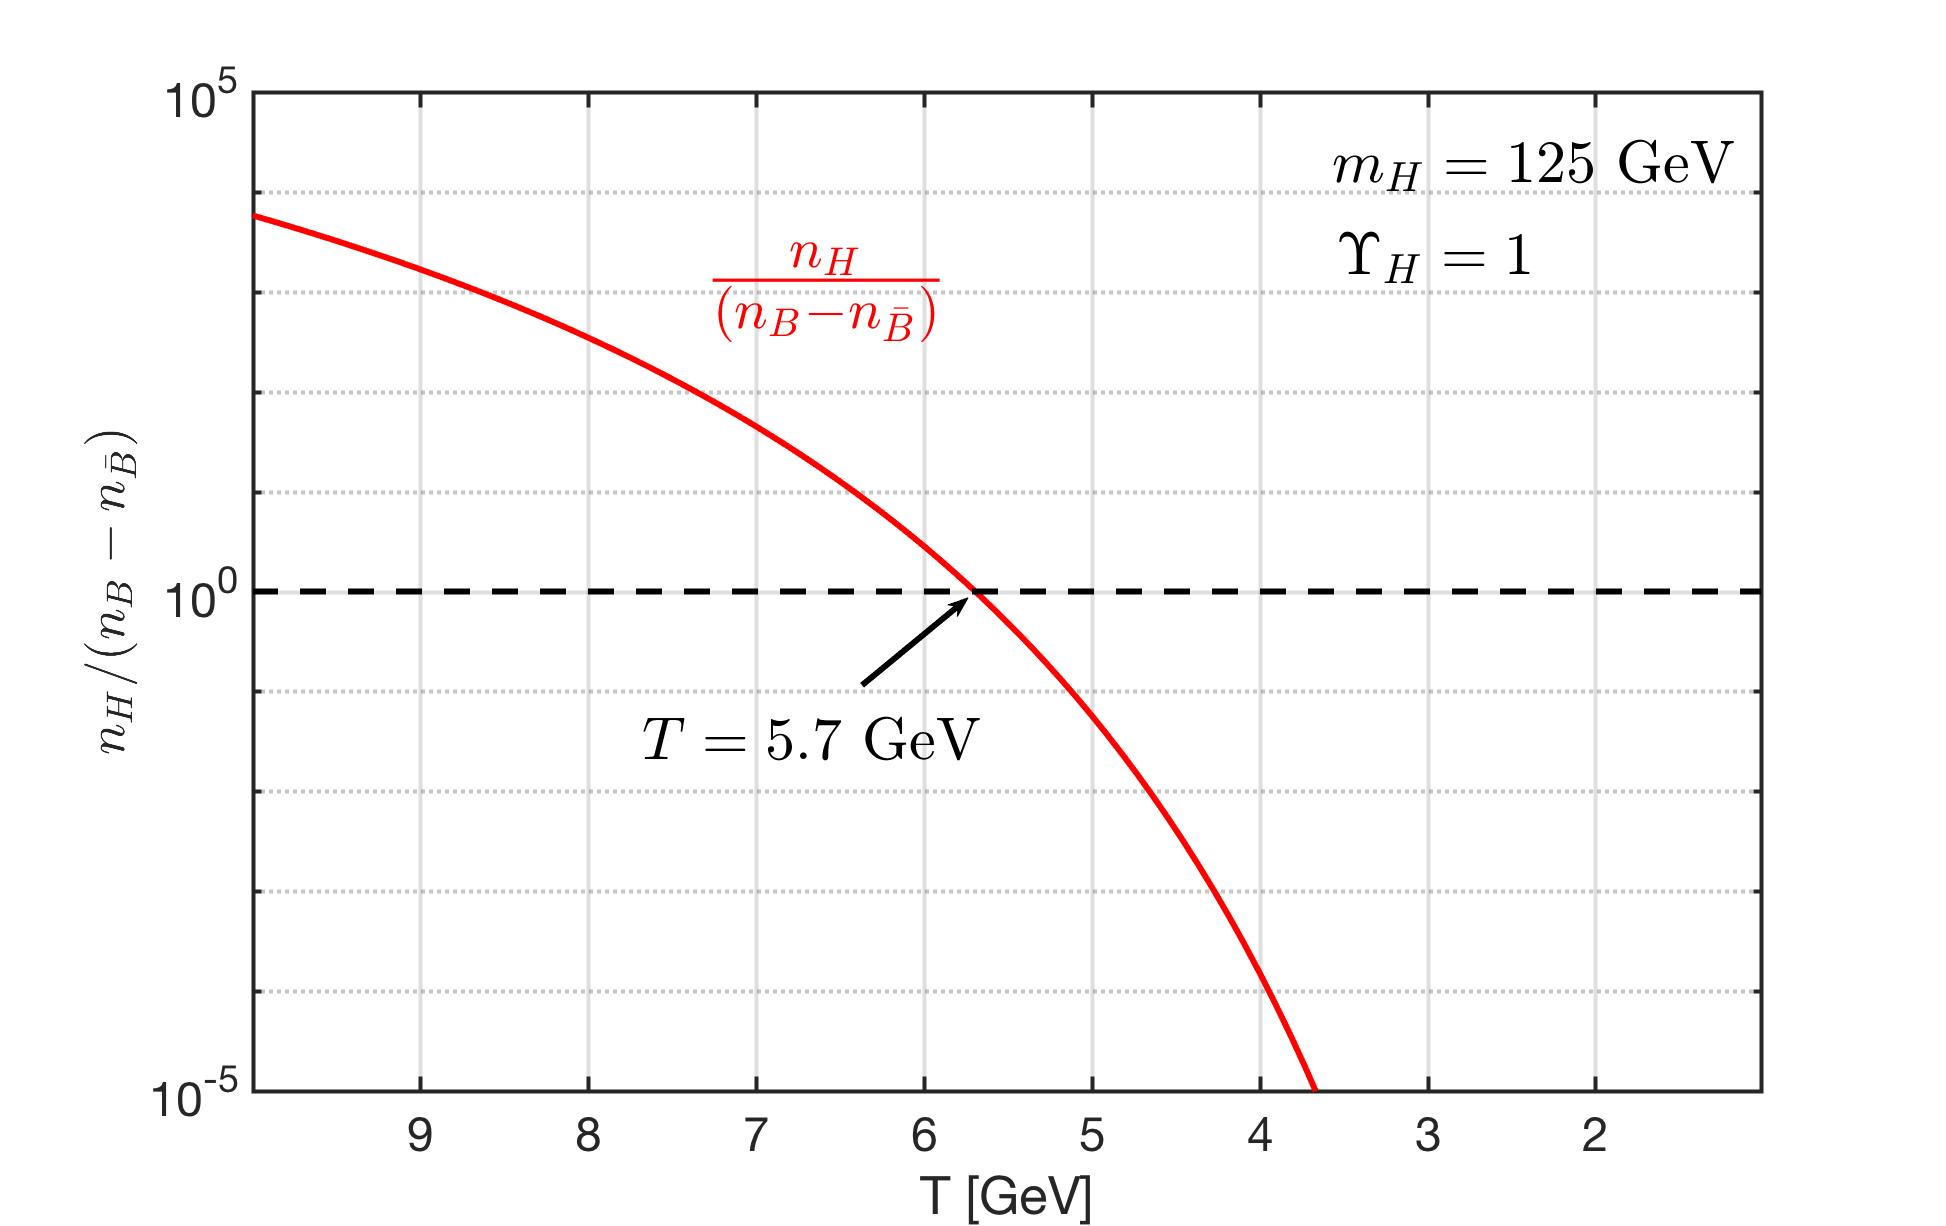
\includegraphics[width=0.9\textwidth]{./plots/HiggsDensityRatio}}
\caption{The ratio between Higgs  density  $n_H$ and baryon asymmetry  density $n_B-n_{\bar B}$ as a function of temperature $T$ assuming chemical Higgs equilibrium $\Upsilon_H=1$. Both densities are equal (horizontal line) at temperature $T=5.7$ GeV}
\label{HiggsDensity_fig} 
\end{figure}
%%%%%%%%%%%%%%%%%%%%%%%%%%%%%%%%%%%%%%%%%%%%%%%%%%%%%%%%%%%%%%%%%%%

%%%%%%%%%%%%%%%%%%%%%%%%%%%%%%%
\paragraph{Production and decay of Higgs in QGP}
In the QGP epoch, the dominant production of the Higgs boson is the bottom quark pair fusion reaction: 
\begin{align}
b+\overline{b}\longrightarrow H\,,
\end{align}
which is the inverse to the important but not dominant decay process of $H\to b+\overline{b}$.

The Higgs predominantly decays via the $W,Z$ decay channels as follows:
\begin{align}
H\longrightarrow WW^\ast\,. ZZ^\ast\longrightarrow\mathrm{anything}\,.
\end{align}
Here $W^\ast,Z^\ast$ represent the production of virtual off-mass-shell gauge bosons decaying rapidly nto  other particle pairs.  Therefore once Higgs decays via this channel at least four particles are rapidly formed and there is no path back for $T\ll m_H$. This is so since the spectral energy of produced particles (which rapidly thermally reequilibrate) is epithermal compared to ambient plasma. 

This qualitative considerations clarify that Higgs will in general not be found in Chemical equilibrium for $T\ll m_H$. We also think that Higgs will not be in kinetic momentum equilibrium, as the production processes will effectively produce a `cold' Higgs particle which given its large mass and negligibel scattering probability with low mass plasma particles will not be able to achieve thermal equilibrium. A dynamic study leading to proper understanding of the off-equilibrium abundance of Higgs and their freeze-out in the early Universe is beyond the scope of this report. 

%%%%%%%%%%%%%%%%%%%%%%%%%%%%%%%%%
\paragraph{Heavy quarks in primordial QGP} 
The primordial quark-gluon plasma (QGP) refers to the state of matter that existed in the early Universe, specifically for time $t\approx 20\, \mathrm{\mu s}$ after the Big Bang. At that time the Universe was controlled by the strongly interacting particles: quarks and gluons. In this chapter, we study the heavy bottom and charm flavor quarks near to the QGP hadronization temperature $0.3\,\mathrm{GeV}>T>0.15\,\mathrm{GeV}$ and examine the relaxation time for the production and decay of bottom/charm quarks then show that the bottom quark nonequliibrium occur near to QGP–hadronization and create the arrow in time in the early Universe.
  
In the QGP epoch, up and down $(u,d)$ (anti)quarks are effectively massless and provide along with gluons, some leptons, and photons the thermal bath defining the thermal temperature. Strange $(s)$ (anti)quarks are also found to be in equilibrium considering their  weak, electromagnetic, and strong interactions, indeed this equilibrium continues in hadronic epoch until $T\approx13$ MeV~\cite{Yang:2021bko}. 

The massive top $(t)$ (anti)quarks couple  to the plasma via the channel~\cite{ParticleDataGroup:2018ovx}
\begin{equation}
t\leftrightarrow W+b\,,\qquad \Gamma_t=1.4\pm0.2\,\mathrm{GeV}\,.
\end{equation}
As is well known, the width prevents formation of bound toponium states. Given the large value of $\Gamma_t$  there is no freeze-out of top quarks until $W$ itself freezes out. To address the top quarks in QGP, a dynamic theory for $W$ abundance is needed, a topic we will embark on in the future. 
 
The semi-heavy bottom $(b)$ and charm $(c)$ quarks can be produced by strong interactions via quark-gluon pair fusion processes, these quarks decay  via weak interaction decays,  their abundance depends on the competition between the strong interaction fusion processes at low temperature inhibited by the mass threshold, and weak decay reaction rates.

In the following we consider the temperature near QGP hadronization $0.3\,\mathrm{GeV}>T>0.15\,\mathrm{GeV}$, and study the bottom and charm abundance by examining the relevant reaction rates of their production and decay.
In thermal equilibrium the number density of light quarks can be evaluated in the massless limit, and we have\index{number density of quark}
\begin{align}\label{FermiN}
n_q=\frac{g_{q}}{2\pi^2}\,T^3 F(\Upsilon_q)\;, \quad F=\int_0^\infty \frac{x^2dx}{1+\Upsilon_q^{-1}e^x}\;,
\end{align}
where $\Upsilon_q$ is the quark fugacity. We have $ F(\Upsilon_q=1)=3\,\zeta(3)/2$ with the Riemann zeta function $\zeta(3)\approx1.202$.
The thermal equilibrium number density of heavy quarks with mass $m\gg T$ can be well described by the Boltzmann expansion of the Fermi distribution function, giving
\begin{align}\label{BoltzN}
n_{q}\!=\!\frac{g_{q}T^3}{2\pi^2}\sum_{n=1}^{\infty}\frac{(-1)^{n+1}\Upsilon_q^n}{n^4}\left(\frac{n\,m_{q}}{T}\right)^{\!2}\!K_2\left(\frac{n\,m_{q}}{T}\right),
\end{align} 
where $K_2$ is the modified Bessel functions of integer order $2$. In the case of interest, when $m\gg T$, it suffices to consider the Boltzmann limit and  keep the first term $n=1$ in the expansion. The first term  $n=1$ also suffices for both charmed $c$-quarks and bottom $b$-quarks, giving
\begin{align}
&n_{b,c}={\Upsilon_{b,c}\,}n^{th}_{b,c},\qquad n^{th}_{b,c}=\frac{g_{b,c}}{2\pi^2}\,T^3\left(\frac{m_{b,c}}{T}\right)^2\,K_2(m_{b,c}/T).
\end{align}
However, for strange $s$ quarks, several terms are needed. 


%%%%%%%%%%%%%%%%%%%%%%%%%%%%%%%%%%%%%%%
\begin{figure}
\centerline{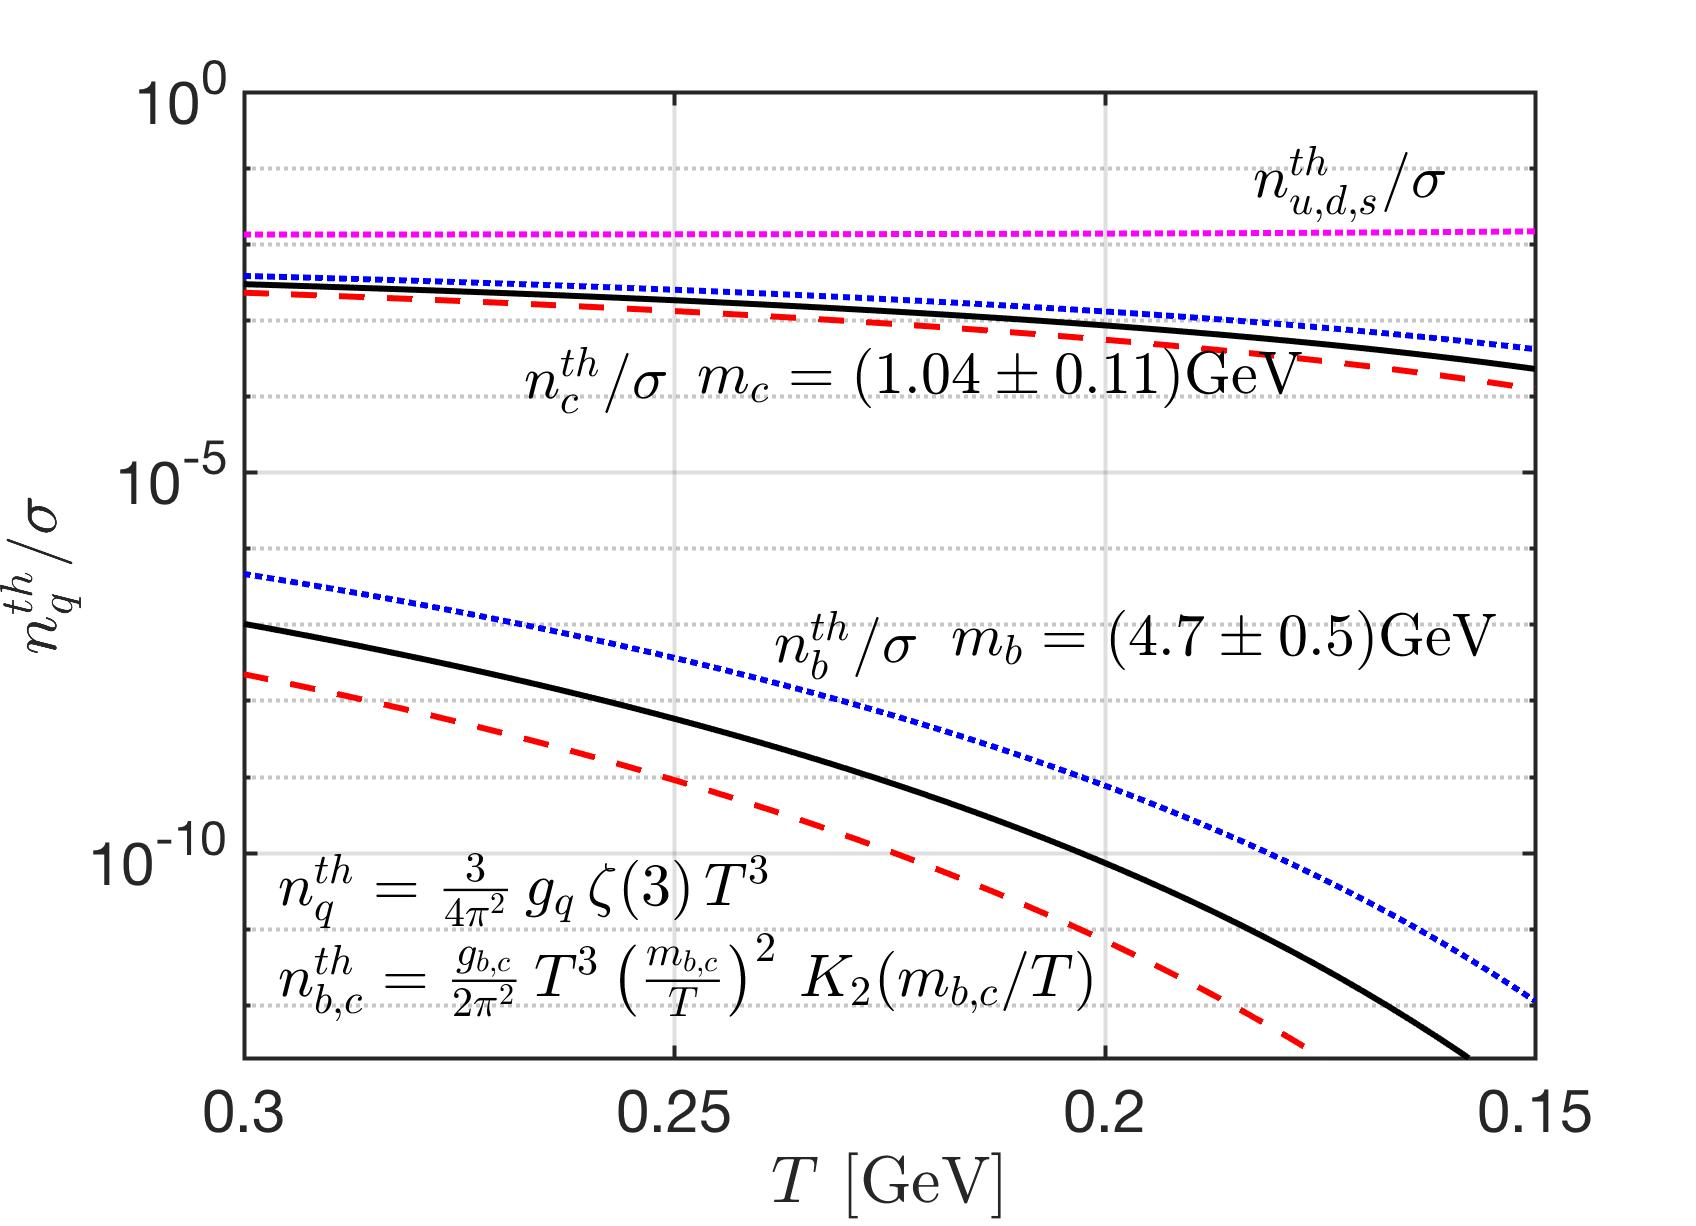
\includegraphics[width=0.9\textwidth]{./plots/bcQuarkDensity_new}}
\caption{
The quark number density normalized by entropy density, as a function of temperature in the early Universe with $\Upsilon=1$. The $b$-quark mass parameters shown are $m_b=4.2\,\mathrm{GeV}$ (blue) dotted line, $m_b=4.7\,\mathrm{GeV}$ (black) solid line, and $m_b=5.2\,\mathrm{GeV}$ (red) dashed line. For  $c$-quark  $m_c=0.93\,\mathrm{GeV}$  (blue) dotted line, $m_c=1.04\,\mathrm{GeV}$ (black) solid line, and $m_c=1.15\,\mathrm{GeV}$ (red) dashed line. Adapted from the thesis of C.T.\,Yang \cite{Yang:2024ret}}
\label{number_entropy_b002} 
\end{figure}
%%%%%%%%%%%%%%%%%%%%%%%%%%%%%%%%%%%%%%%%%%% 

In \rf{number_entropy_b002} we show the equilibrium ($\Upsilon=1$) number density per entropy density  ratio as a function of temperature $T$ of quarks. The entropy density is given by \req{entropy} and only light particles contribute to the entropy density; thus the result we consider is independent of actual abundance of $c$, $b$ and other heavy particles. We evaluated the density-per-entropy ratio for  $m_b=4.2,\;4.7,\;5.2$\,GeV and $m_c=1.04\pm0.11$\,GeV. The $m_b\simeq 5.2\,\mathrm{GeV}$ is  a typical potential model mass used in modeling bound states of bottom, and $m_b=4.2,\,4.7\,\mathrm{GeV}$ is the current quark mass at low and high energy scales. In \rf{number_entropy_b002} we see that the charm abundance in the domain of interest $0.3\,\mathrm{GeV}>T>0.15\,\mathrm{GeV}$ is about $10^4\sim\!\!10^{9}$ times greater than the bottom quarks. This implies that the small $b$,$\bar b$ quark abundance is embedded in a large background comprising all lighter $u,d,s,c$ quarks and antiquarks, as well as gluons $g$.

%%%%%%%%%%%%%%%%%%%%%%%%%%%%%%%%%%%%%
\paragraph{Hubble expansion rate}
In the early Universe, within a temperature range $130\, \mathrm{GeV}>T>0.15\,\mathrm{GeV}$,  we have the following particles:  photons, $8$ color charge gluons, $W^\pm$, $Z^0$, three generations of $3$ color charge quarks and leptons in the primordial QGP.  The Hubble parameter can be written in terms of particle energy density $\rho_i$
\begin{align}
H^2=\frac{8\pi G_N}{3}\left(\rho_\gamma+\rho_{\mathrm{lepton}}+\rho_{\mathrm{quark}}+\rho_{g,{W^\pm},{Z^0}}\right),
\end{align}
where $G_N$ is the Newtonian constant of gravitation. The effectively massless particles and radiation dominate the speed of expansion of the Universe. The characteristic Universe expansion time constant $1/H$ is seen in \rf{BCreaction_fig}. In the epoch of interest to us $0.3\,\mathrm{GeV}>T>0.15\,\mathrm{GeV}$, the Hubble time $1/H\approx10^{-5}$ sec which is much longer than the lifespan and production time of the bottom and charm quarks. 

%%%%%%%%%%%%%%%%%%%%%%%%%%%%%%%%
\subsection{Reaction rates for heavy quark  production and decay}
In primordial QGP, the bottom and charm quarks can be produced from strong interactions via quark-gluon pair fusion processes and disappear via weak interaction decays. For production, we have the following processes
\begin{align}
 q+\bar{q}&\longrightarrow b+\bar b,\qquad q+\bar{q}\longrightarrow c+\bar c,\\
 g+g&\longrightarrow b+\bar b,\qquad g+g\longrightarrow c+\bar c,
\end{align}
for bottom and charm we have
\begin{align}
 &b\longrightarrow c+l+\overline{\nu_l}, \qquad b\longrightarrow c+q+\bar{q},\\
&c\longrightarrow s+l+\overline{\nu_l},\qquad c\longrightarrow s+q+\bar{q},
\end{align}
for their decay. In following we will calculate the production rate and decay rate for bottom and charm quarks and compare to the Universe expansion rate. We will show that in the epoch of interest to us the characteristic Universe expansion time $1/H$ is much longer than the lifespan and production time of the bottom/charm quark. In this case, the dilution of bottom/charm quark due to the Universe expansion is slow compare to the the strong interaction production, and the weak interaction decay of the bottom/charm. 
 


%%%%%%%%%%%%%%%%%%%%%%%%%%%%%%%%%%%%%
\paragraph{Quark production rate via strong interaction}
For the quark-gluon pair fusion processes\index{bottom quark!production rate}
%\begin{align}
% q+q&\longrightarrow b+\bar b,\qquad q+q\longrightarrow c+\bar c,\\
% g+g&\longrightarrow b+\bar b,\qquad g+g\longrightarrow c+\bar c,
%\end{align}
the evaluation of the lowest-order Feynman diagrams yields the cross sections~\cite{Letessier:2002ony}:
\begin{align}
&\sigma_{q\bar{q}\rightarrow b\bar{b},c\bar{c}}=\frac{8\pi\alpha_s^2}{27s}\left(1+\frac{2m_{b,c}^2}{s}\right)w(s),\,\qquad w(s)=\sqrt{1-{4m^2_{b,c}}/{s}},\\
&\sigma_{gg\rightarrow b\bar{b},c\bar{c}}=\!\frac{\pi\alpha_s^2}{3s}\bigg[\left(1\!+\!\frac{4m^2_{b,c}}{s}\!+\!\frac{m^4_{b,c}}{s^2}\right)\ln{\left(\frac{1+w(s)}{1-w(s)}\right)}\!-\!\left(\frac{7}{4}\!+\!\frac{31m^2_{b,c}}{4s}\right)w(s)\bigg],
\end{align} 
where $m_{b,c}$ represents the mass of bottom or charm quark, $s$ is the Mandelstam variable, and $\alpha_s$ is the QCD coupling constant. Considering the perturbation expansion of the coupling constant $\alpha_s$ for the two-loop approximation~\cite{Letessier:2002ony}, we have:
\begin{align}
\alpha_s(\mu^2)=\frac{4\pi}{\beta_0\ln({\mu^2/\Lambda^2})}\bigg[1-\frac{\beta_1}{\beta_0}\frac{\ln(\ln{(\mu^2/\Lambda^2)})}{\ln(\mu^2/\Lambda^2)}\bigg],
\end{align}
where $\mu$ is the renormalization energy scale and $\Lambda^2$ is a parameter that determines the strength of the interaction at a given energy scale in QCD. The energy scale we consider is based on required gluon/quark collisions above $b\bar b$ energy threshold, so we have $\mu=2m_b+T$. For the energy scale $\mu>2m_b$ we have $\Lambda=180\sim230$ MeV( $\Lambda\approx205$ MeV in our calculation), and the parameters $\beta_0=11-2n_f/3$, $\beta_1=102-38n_f/3$ with the number of active fermions $n_f=4$. 

In general the thermal reaction rate per unit time and volume $R$ can be written in terms of the scattering cross section as follows~\cite{Letessier:2002ony}:
\begin{align}
R\equiv\sum_i\int_{s_{th}}^\infty\!ds\,\frac{dR_i}{ds}=\sum_i\int_{s_{th}}^\infty\!ds\,\sigma_i(s)\,P_i(s),
\end{align}
where $\sigma_i(s)$ is the cross section of the reaction channel $i$, and $P_i(s)$ is the number of collisions per unit time and volume. Considering the quantum nature of the colliding particles (i.e., Fermi and Bose distribution) with the massless limit and chemical equilibrium condition ($\Upsilon=1$), we obtain~\cite{Letessier:2002ony}
\begin{align}
&P_i(s)=\frac{g_1g_2}{32\pi^4}\,\frac{T}{1+I_{12}}\frac{\lambda_2}{\sqrt{s}}\!\sum_{l,n=1}^{\infty}\!(\pm)^{l+n}\frac{K_1(\sqrt{lns}/T)}{\sqrt{ln}},\\
&\lambda_2\equiv\left[s-\left(m_1+m_2\right)^2\right]\,\left[s-\left(m_1-m_2\right)^2\right],
\end{align}
where $+$ is for boson and $-$ is for fermions, and the factor $1/(1+I_{12})$ is introduced to avoid double counting of indistinguishable pairs of particles. $I_{12}=1$ for identical pair of particles, otherwise $I_{12}=0$. Hence the total thermal reaction rate per volume for bottom quark production can be written as
\begin{align}
\label{Bquark_Source}
R^{\mathrm{Source}}_{b,c}=\int^\infty_{s_{th}}ds\,\bigg[\sigma_{q\bar{q}\rightarrow b\bar{b},c\bar{c}}\,P_q+\sigma_{gg\rightarrow b\bar{b},c\bar{c}}\,P_g\bigg]%=R_{q\bar{q}\rightarrow b\bar{b},c\bar{c}}+R_{gg\rightarrow b\bar{b},c\bar{c}}.
\end{align}
We introduce the bottom/charm quark relaxation time for the quark-gluon pair fusion as follows:
\begin{align}
\label{relaxation_time}
&{\tau_{b,c}^{\mathrm{Source}}}\equiv\frac{dn_{b,c}/d\Upsilon_{b,c}}{R^{\mathrm{Source}}_{b,c}}\;,\quad
\end{align}
where $dn_{b,c}/d\Upsilon_{b,c}=n^{th}_{b,c}$ in the Boltzmann approximation. The relaxation time is on the order of magnitude of time needed to reach chemical equilibrium. In \rf{BCreaction_fig} we show the characteristic time for bottom/charm  quark strong interaction production in the domain of interest, $ 0.3\,\mathrm{GeV}>T> 0.15\,\mathrm{GeV}$. 

%%%%%%%%%%%%%%%%%%%%%%%%%%%%%%%%
\paragraph{Quark decay rate via weak interaction}
The bottom/charm quark decay via the weak interaction.\index{bottom quark!decay rate}
%\begin{align}
% &b\longrightarrow c+l+\nu_l, \qquad %b\longrightarrow c+q+\bar{q},\\
%&c\longrightarrow s+l+\nu_l,\qquad c\longrightarrow s+q+\bar{q},
%\end{align}
The vacuum decay rate for $1\to2+3+4$ in vacuum can be evaluated via the weak interaction:
\begin{align}
\frac{1}{\tau_1}=&\frac{64G^2_F\,V^2_{12}\,V^2_{34}}{(4\pi)^3g_1}\,m^5_1\times\left[\frac{1}{2}{\left(1-\frac{m^2_2}{m^2_1}-\frac{m^2_3}{m^2_1}+\frac{m^2_4}{m^2_1}\right)}\mathcal{J}_1-\frac{2}{3}\mathcal{J}_2\right],
\end{align}
where the Fermi constant is $G_F=1.166\times10^{-5}\,\mathrm{GeV}^{-2}$, $V_{ij}$ is the element of the Cabibbo-Kobayashi-Maskawa (CKM) matrix~\cite{Czarnecki:2004cw} for quark channel and $V_{l\nu_l}=1$ for lepton channel. The functions $\mathcal{J}_1$ and $\mathcal{J}_2$ are given by
\begin{align}
&\mathcal{J}_1\!=\!\!\!\int_0^{(1-m^2_2/m^2_1)/2}\!\!\!\!\!\!\!\!dx\left(1\!-\!2x\!-\!\frac{m^2_2}{m_1^2}\right)^{\!\!2}\left[\frac{1}{(1-2x)^2}-1\right]\\
&\mathcal{J}_2\!=\!\!\!\int_0^{(1-m^2_2/m^2_1)/2}\!\!\!\!\!\!\!\!dx\left(1\!-\!2x\!-\!\frac{m^2_2}{m_1^2}\right)^{\!\!3}\left[\frac{1}{(1-2x)^3}-1\right]
\end{align}
The modification due to the heat bath(plasma) is small because the bottom and charm  mass $m_{b,c}\gg T$~\cite{Kuznetsova:2008jt}. In the temperature range we are interested in, the decay rate in the vacuum is a good approximation for our calculation. We show the lifespan for bottom/charm quark in \rf{BCreaction_fig}. 

%there is no modification due to the phase space blocking because the bottom/charm mass is too heavier $m_{b,c}\gg T$~\cite{Kuznetsova:2008jt}. We did not include above either base enhancement nor fermi blocking factors since process of bottom decay involve energies beyond those available for $ 150< T< 300\,\mathrm{MeV}$.



%%%%%%%%%%%%%%%%%%%%%%%%%%%%%%%%%%%%%%%
\begin{figure}  
\centerline{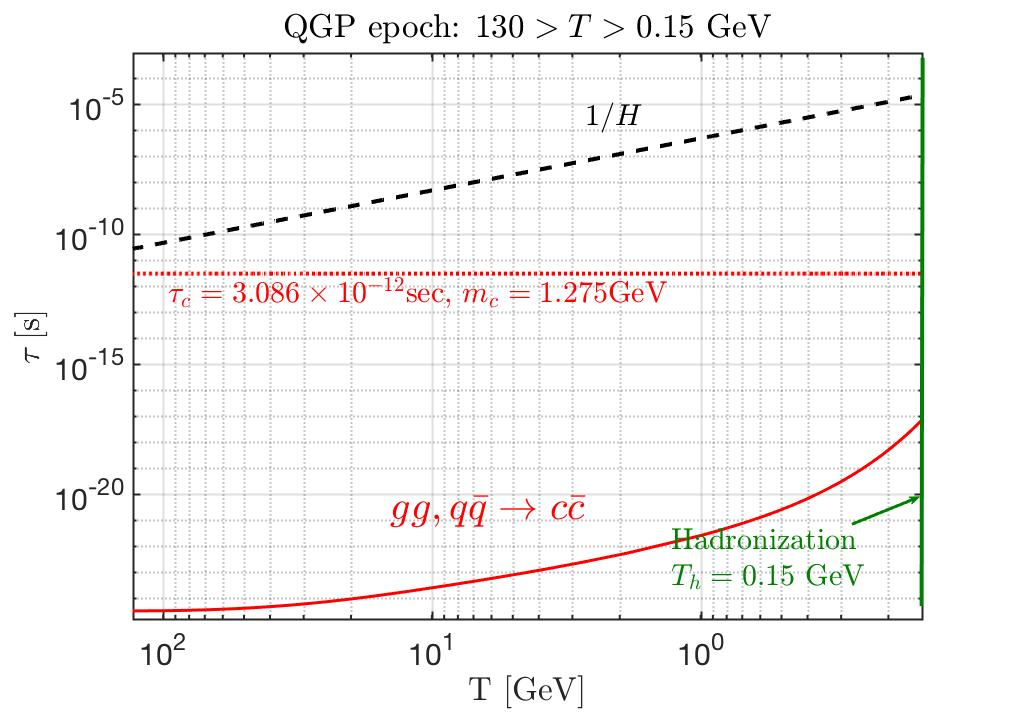
\includegraphics[width=0.9\textwidth]{./plots/CharmQuark_QGP.jpg}}
\centerline{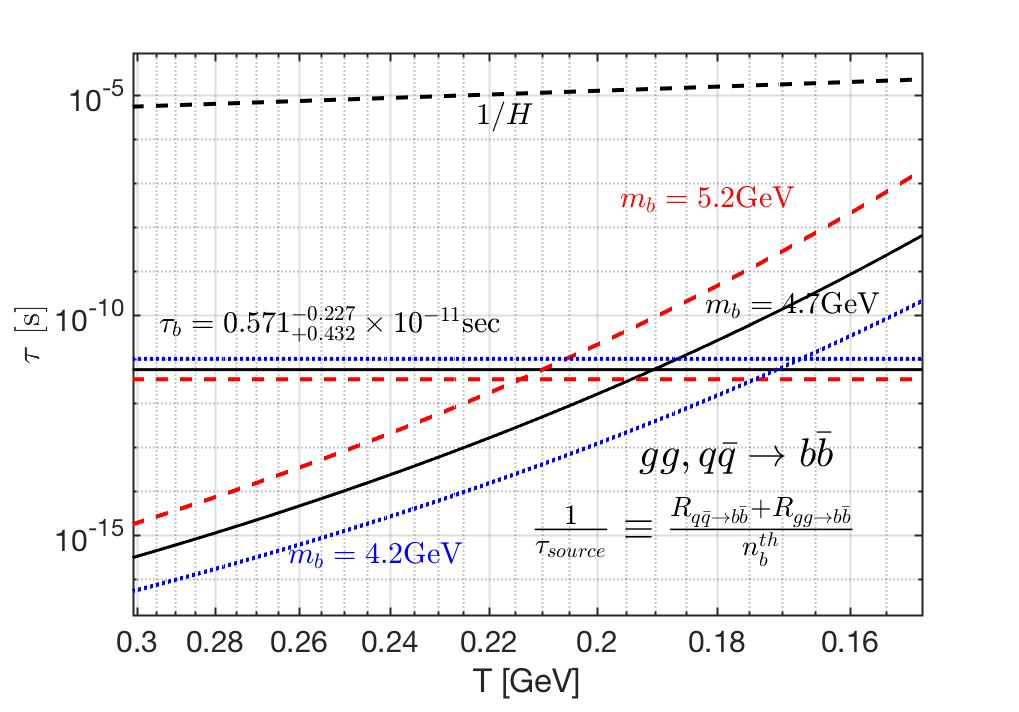
\includegraphics[width=0.9\textwidth]{./plots/BQuarkReactionTime_bottom.jpg}}
\caption{\cccite{Rafelski:2023emw}, adapted from thesis of C.T.\,Yang \cite{Yang:2024ret}. Comparison of Hubble time $1/H$, quark lifespan $\tau_{q}$, and characteristic time for production via quark-gluon pair fusion for (top figure) charm and (bottom figure) bottom quarks as a function of temperature. Both figures end at approximately the hadronization temperature of $T_{H}\approx150$ MeV. Three different masses $m_{b}=4.2$ GeV (blue short dashes), $4.7$ GeV, (solid black), $5.2$ GeV (red long dashes) for bottom quarks are plotted to account for its decay width}
\label{BCreaction_fig}
\end{figure}
%%%%%%%%%%%%%%%%%%%%%%%%%%%%%%%%%%%%%%%



 

%%%%%%%%%%%%%%%%%%%%%%%%%%%%%%%%%%%%%%%%%%%%%
\paragraph{Rate Comparison: Strong fusion, Weak decay, and Hubble expansion}
%%%%%%%%%%%%%%%%%%%%%%%%%%%%%%%%%%%%%
%\paragraph{Hubble expansion rate}
In the early Universe, within a temperature range $130\, \mathrm{GeV}>T>0.15\,\mathrm{GeV}$,  we have the following particles:  photons, $8$ color charge gluons, $W^\pm$, $Z^0$, three generations of $3$ color charge quarks and leptons in the primordial QGP.  The Hubble parameter can be written in terms of particle energy density $\rho_i$
\begin{align}
H^2=\frac{8\pi G_N}{3}\left(\rho_\gamma+\rho_{\mathrm{lepton}}+\rho_{\mathrm{quark}}+\rho_{g,{W^\pm},{Z^0}}\right),
\end{align}
where $G_N$ is the Newtonian constant of gravitation. The effectively massless particles and radiation dominate the speed of expansion of the Universe. The characteristic Universe expansion time constant $1/H$ is seen in \rf{BCreaction_fig}. In the epoch of interest to us $0.3\,\mathrm{GeV}>T>0.15\,\mathrm{GeV}$, the Hubble time $1/H\approx10^{-5}$ sec which is much longer than the lifespan and production time of the bottom and charm quarks. 

In \rf{BCreaction_fig} (top), we plot the relaxation time of the production/decay for charm quarks and Hubble time $1/H$ as a function of temperature. Throughout the entire duration of QGP, the Hubble time is larger than the lifespan and production times of the charm quark. %Therefore, the heavy charm quark remains in equilibrium as its processes occur faster than the expansion of the Universe. 
Additionally, the charm quark production time is faster than the decay. The faster quark-gluon pair fusion keeps the charm in chemical equilibrium up until hadronization. After hadronization, charm quarks form heavy mesons that decay into multi-particles quickly in plasma. The daughter particles from charm meson decay can interact and reequilibrate with
the plasma quickly. In this case the energy required for the inverse decay reaction to produce
charm meson is difficult to overcome and causing the charm quark to vanish from the inventory of particles via decay in the Universe.

In \rf{BCreaction_fig} (bottom) we present the relaxation times for production and decay of the bottom quark with different masses as a function of temperature. It shows that both production and decay are faster than the Hubble time $1/H$ for the duration of QGP. However, unlike charm quarks, the relaxation time for bottom quark production intersects with bottom quark decay at different temperatures which depends on the mass of the bottom. The intersection implies that the bottom quark freeze-out from the primordial plasma before hadronization as the production process slows down at low temperatures and the subsequent weak interaction decay leads to a dilution of the bottom quark content within the QGP plasma. All of this occurs with rates faster than Hubble expansion and thus as the Universe expands, the system departs from a detailed chemical balance because of the competition between decay and production reactions in QGP. In this scenario, the dynamic equation on bottom abundance is required and causes the distribution to deviate from equilibrium with $\Upsilon\neq1$ in the temperature range below the crossing point but before the hadronization. 



%%%%%%%%%%%%%%%%%%%%%%%%%%%%
\subsection{Is baryongenesis possible in QGP phase?}\label{Bottom}
%%%%%%%%%%%%%%%%%%%%%%%%%%%%%%%%%%%%%%%%%%%%
\paragraph{Bottom quark abundance nonequilibrium}\index{bottom quark!nonequilibrium}
The competition between weak interaction decay and strong interaction production rates  can lead  to a non-equilibrium dynamic heavy quark abundance. We explore as example the case of bottom quarks  in QGP we explore. Similar considerations apply to all heavier PP-SM particles including in particular  Higgs, W,Z gauge bosons, top $t$ quark. 
 
The dynamic equation for bottom quark abundance in QGP can be written as \index{bottom quark!population equation}
\begin{align}
\label{Bquark_eq}
\frac{1}{V}\frac{dN_b}{dt}=\big(\,1-\Upsilon^2_{b}\,\big)\,R^{\mathrm{Source}}_{b}-\Upsilon_b\,R^{\mathrm{Decay}}_{b}\;,
\end{align}
where $R^{\mathrm{Source}}_{b}$ and $R^{\mathrm{Decay}}_{b}$ are the thermal reaction rates per volume of production and decay of bottom quark, respectively. The bottom source rates are the gluon and quark fusion rates \req{Bquark_Source}. The decay rate depends on whether the bottom quarks are freely present in the plasma or are bounded within mesons. We consider two extreme scenarios for the bottom quark population: 1.) all bottom flavor is free, and 2.) all bottom flavor is bounded into mesons in QGP. In \rf{ReactionTime}  we show the characteristic interaction times relevant to the abundance of bottom quarks, as well as the Hubble time $1/H$ for the temperature range of interest, $0.3\,\mathrm{GeV}> T> 0.15\,\mathrm{GeV}$.

%%%%%%%%%%%%%%%%%%%%%%%%%%%%%%%%%%%%%%
\begin{figure} 
\centerline{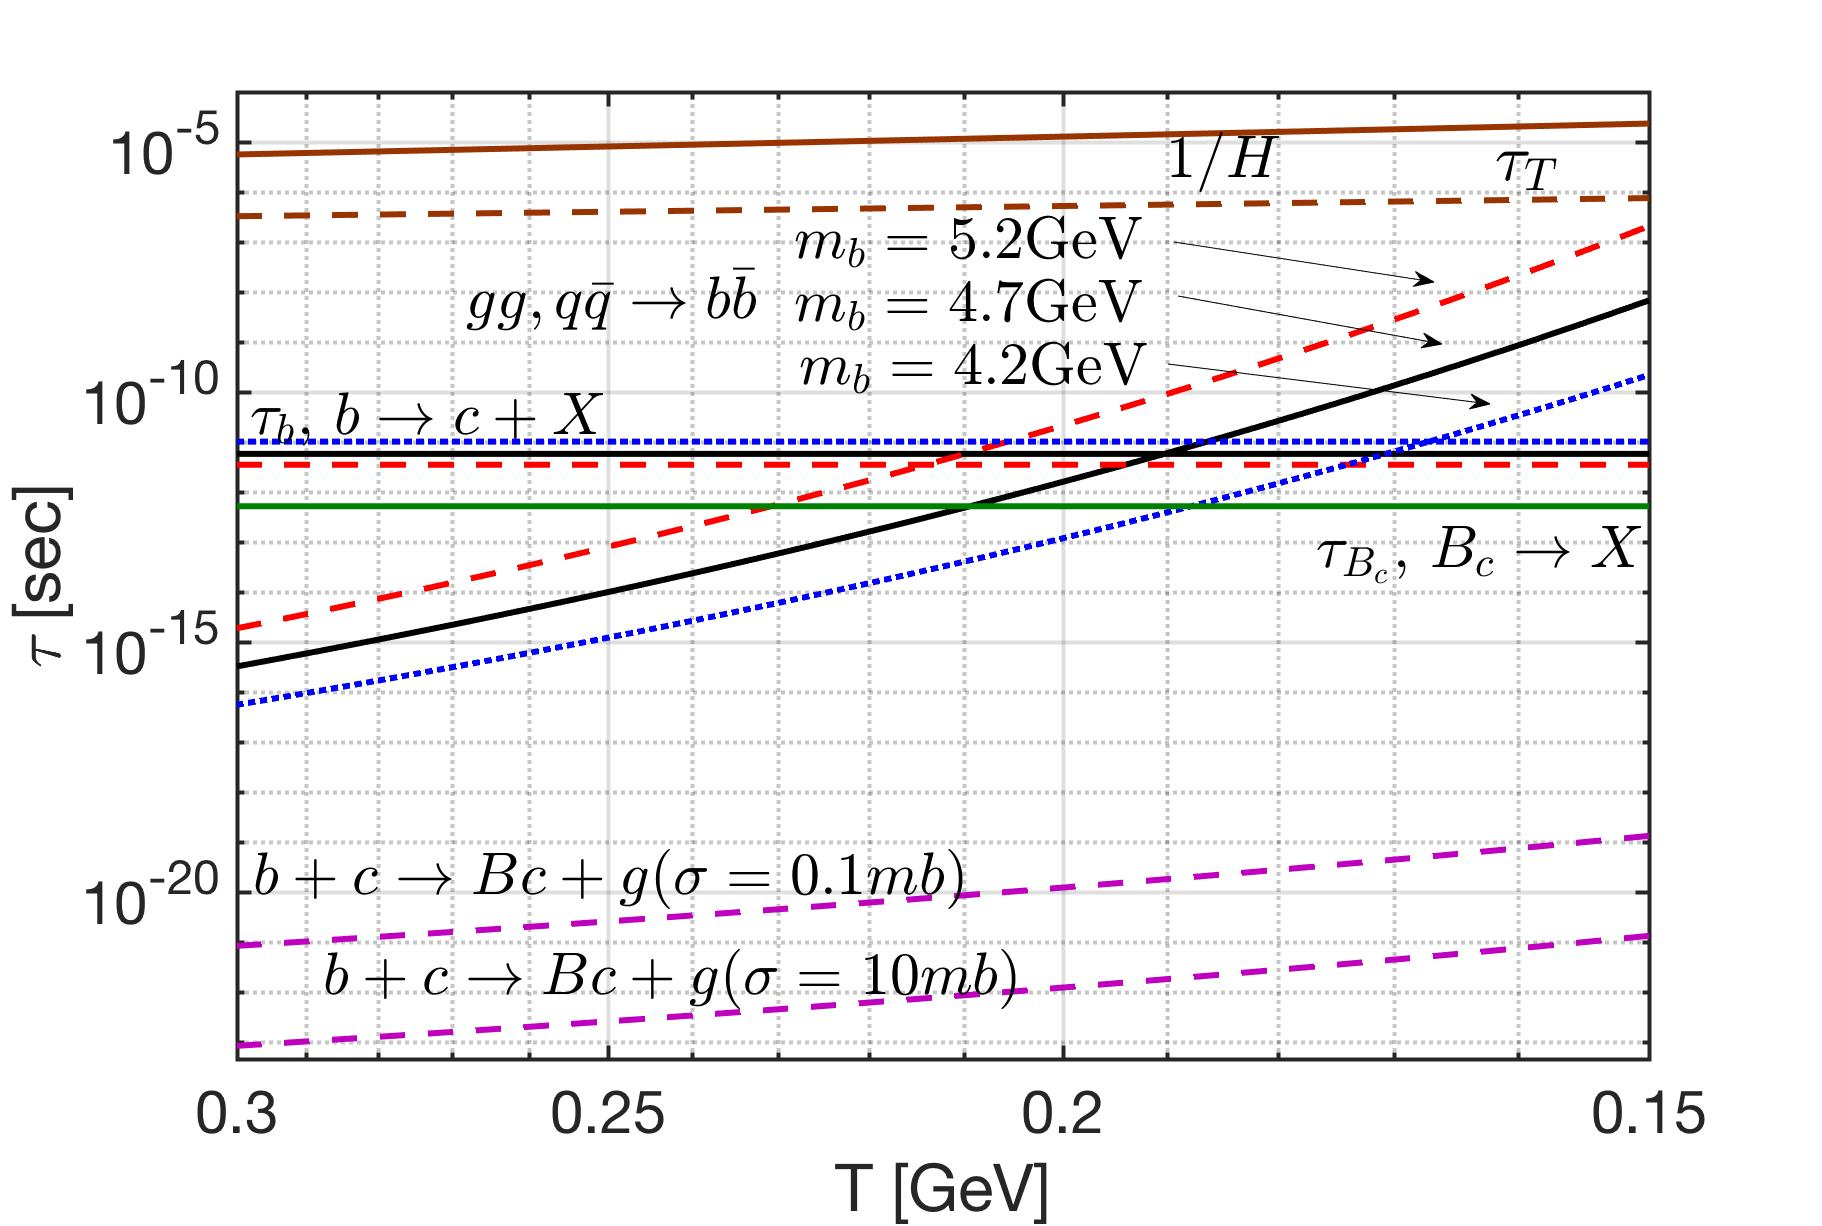
\includegraphics[width=0.9\textwidth]{./plots/BQuarkReactionTime003}}
\caption{Characteristic production, decay, times of bottom quark  as a function of  temperature $T$ for $0.3\,\mathrm{GeV}>T> 0.15\,\mathrm{MeV}$.  Near the top of figure  $1/H$ (brown solid line) and $\tau_T$ (brown dashed line); other horizontal lines are bottom-quark (in QGP) weak interaction lifetimes $\tau_b$ for the three different masses: $m_b=4.2\,\mathrm{GeV}$ (blue dotted line), $m_b=4.7\,\mathrm{GeV}$ (black solid  line), $m_b=5.2\,\mathrm{GeV}$ (red dashed line), and the vacuum lifespan $\tau_B$ of the  B$_c$ meson (green solid  line). The relaxation time for strong interaction bottom production $g+g, q+\bar q\rightarrow b+\bar{b}$ is shown with three different bottom masses and same type-color coding as weak interaction decay rate. At bottom of figure the in plasma formation process (dashed lines, purple) $b+c\rightarrow \mathrm{B}_c+g$ with cross section range $\sigma=0.1,10\,\mathrm{mb}$. Adapted from the thesis of C.T.\,Yang \cite{Yang:2024ret}}
\label{ReactionTime}
\end{figure}
%%%%%%%%%%%%%%%%%%%%%%%%%%%%%%%%%

Considering all bottom flavor is free in QGP, the bottom decay rate per volume is the bottom lifespan weighted with density of particles \req{BoltzN}, see Ref.\,\cite{Kuznetsova:2008jt}. We have
\begin{align}\hspace{0.5cm}
R^{\mathrm{Decay}}_b=\frac{dn_b/d\Upsilon_b}{\tau_b},\,\,\,\,\, \tau_b\approx0.57\times10^{-11} \mathrm{sec}.
\end{align}
On the other hand, $b$,$\bar b$ quark abundance is embedded in a large background comprising all lighter quarks and antiquarks (see \rf{number_entropy_b002}). After formation the heavy $b, \bar b$ quark can bind with any of the available lighter quarks, with the most likely outcome being a chain of reactions 
\begin{align}
&b+q\longrightarrow\mathrm{B}+g\;,\\
&\mathrm{B}+s\longrightarrow\mathrm{B}_s+q\;,\\
&\mathrm{B}_s+c\longrightarrow\mathrm{B}_c+s\;,
\end{align}
with each step providing a gain in binding energy and reduced speed due to the diminishing abundance of heavier quarks $s, c$. To capture the lower limit of the rate of $\mathrm{B}_c$ production we show in \rf{ReactionTime} the expected formation rate by considering the direct process $b+\overline c\rightarrow \mathrm{B}_c+g$, considering the range of cross section $\sigma=0.1\sim10\,\mathrm{mb}$ ~\cite{Schroedter:2000ek}. The rapid formation rate of B$_c(b\bar c)$ states in primordial plasma is shown by purple dashed lines at bottom in \rf{ReactionTime}, we have
\begin{align}
\tau (b+\overline c\rightarrow \mathrm{B}_c+g)\approx(10^{-16}\sim10^{-14})\times\frac{1}{H} \;.
\end{align}

Despite the low abundance of charm, the rate of $\mathrm{B}_c$ formation is relatively fast, and that of lighter flavored B-mesons is substantially higher. Note that as long as we have bottom quarks made in gluon/quark fusion bound practically immediately with any quarks $u, d, s$ into B-mesons, we can use the production rate of $b, \bar b$ pairs as the rate of B-meson formation in the primordial-QGP, which all decay with lifespan of pico-seconds. We believe that this process is fast enough to allow consideration of bottom decay from the B$_c(b\bar c)$, $\overline{\mathrm{B}}_c(\bar b c)$ states~\cite{Yang:2020nne}.  
 Based on the hypothesis that all bottom flavor is bound rapidly into $\mathrm{B}_c^\pm$ mesons, we have 
\begin{align}\label{Bc_source}
g+g, q+q \longleftrightarrow &b+\bar b\;[b(\bar{b})+\bar{c}(c)]\longrightarrow \mathrm{B}_c^\pm\longrightarrow\mathrm{anything}.
\end{align}
In this case, the decay rate per volume can be written as
\begin{align}\hspace{0.5cm}
 R^{\mathrm{Decay}}_b=\frac{dn_b/d\Upsilon_b}{\tau_{\mathrm{B}_c}},\,\,\,\,\, \tau_{\mathrm{B}_c}\approx0.51\times10^{-12} \mathrm{sec}.
 \end{align}

%%%%%%%%%%%%%%%%%%%%%%%%%%%%
\paragraph{Baryon asymmetry and Sakhraov conditions}
From the PDG, the observed baryon-to-photon density ratio $\eta$ today is given by  $5.8\times10^{-10} \leqslant\eta\leqslant6.5\times10^{-10}$ \cite{ParticleDataGroup:2018ovx} where the $\eta=(6.12\pm0.04)\times10^{-10}$~\cite{ParticleDataGroup:2022pth} is used in our calculation. This observed value is the evidence of baryon asymmetry and quantifies the matter-antimatter asymmetry in the Universe.

The small value of the baryon asymmetry could be interpreted as simply due to the initial conditions in the Universe. However, in the current standard cosmological model, it is believed that the inflation event can erase any pre-existing asymmetry between baryons and anti-baryons. In this case, we need a dynamic baryogenesis process to generate excess of baryon number compared to anti-baryon number in order to create the observed baryon number today.

The precise epoch responsible for the observed matter genesis $\eta$  in the early Universe has not been established yet.  Several mechanisms have been proposed to explain baryogenesis with investigations typically focusing on the temperature range between GUT phase transition $T_\mathrm{G}\simeq10^{16}\,\mathrm{GeV}$ and the electroweak phase transition near $T_\mathrm{W}\simeq130\,\mathrm{GeV}$~\cite{Kuzmin:1985mm,Kuzmin:1987wn,Arnold:1987mh,Kolb:1996jt,Riotto:1999yt,Nielsen:2001fy,Giudice:2003jh,Davidson:2008bu,Morrissey:2012db}.

In following  we present arguments that the Sakharov conditions~\cite{Sakharov:1967dj} for matter asymmetry to form also appear during QGP era and by example show the possibility that bottom catalyzed the baryongenesis. However, it appears that other heavy particles including the Higgs as described above can fullfill nonequilibrium requirement. So our bottom case maybe just the proverbial tip of an iceberg.

In 1967, Andrei Sakharov  formulated the three conditions necessary to permit baryogenesis in the early Universe~\cite{Sakharov:1967dj} and in 1991 he refined the three conditions as follows~\cite{Sakharov:1988vdp}:
\begin{itemize}
  \item Absence of baryonic charge conservation 
  \item Violation of CP-invariance
  \item Non-stationary conditions in absence of local thermodynamic equilibrium
\end{itemize}
 
In regard to first Sakharov condition: There is a clear assumption that there is no initial asymmetry in baryon number in the Universe. Toady it is argued an initial asymmetry could not survive the  inflationary expansion. Furthermore ad-hoc Big-Bang  baryon-antibaryon inherent asymmetry seems less attractive.  In short we believe that the asymmetry between baryons and anti-baryons we observe requires  the presence of baryon number non-conserving reactions. The other option, an interaction which  favors agglomerations of same `sign' baryonic matter creating large domains in the Universe with small baryon-antibaryon asymmetry has never taken hold: We recall that the opposite is true, elementary antimatter is eclectically attracted to matter. Neutral composite baryonic particles present in era in which antimatter is present (e.g. neutrons, $|Lambda(uds)$, charmed baryons etc emerging just after QGP hadronization) deserve a 2nd look on this account but we do not want to raise any hopes. 

The second Sakharov condition requiring $CP$ violation assures us that we can recognize in universal manner the difference between matter and antimatter.  Clearly, we  could not enhance one form with reference to the other without being able to tell  of matter from antimatter.  CP violation is  allowing us to share with another distant civilization that we are made of matter. A nice textbook discussion showing how to do this using Kaon system CP violation is offered by Perkins~\cite{Perkins:1982xb}.

The third  Sakharov condition is a requirement for breaking of detailed balance condition: It is evident that in thermal equilibrium, the net effect of baryogenesis processes is cancelled out by the detailed balance between  forward and back-reactions. Space-time domains involving phase transitions harbor non-equilibrium thermal distributions  leading to breaking of detailed balance. So far efforts to create consistent description of baryogenesis based on electro-weak phase transition near $T=130$\,GeV has not been able to generate the observed baryon asymmetry. 

We distinguish kinetic (momentum distribution) and chemical (particle abundance) equilibrium. This is so since kinetic equilibrium is usually established much more quickly, while abundance yields are more difficult to establish, especially so for particles with masses in excess, or at least similar to ambient temperatures~\cite{Koch:1986ud,Birrell:2014gea}. This distinction has two relevant consequences: a) Detailed balance can arise  also outside of strict thermal equilibrium condition which is seen in other physical environments, including the nucleo-synthesis processes in the Universe (BBN) and stars.  b) There is a long lasting small violation of detailed balance related to the arrow of time introduced by the Universe expansion. 

Specifically for all heavy primordial particles including the top $t$ and bottom $b$ quarks, W and Z gauge bosons, and, the Higgs particle H we observe that when the Universe expands and temperature cools down well below the particle mass, the production process and decay processes create a stationary equilibrium with detailed balance outside of equilibrium at a fixed temperature. However, Universe expansion disturbs this creating non-stationary effects. Thus we interpret the third condition of Sakharov in our specific context as follows:
\begin{itemize}
\item Non-stationary conditions in absence of local thermodynamic equilibrium $\Longrightarrow$  Absence of detailed balance associated with non-equilibrium yields and non-stationary particle abundance evolution.
\end{itemize} 
We believe that the presence of chemical (abundance) non-equilibrium is thus equally relevant for baryogenesis and can create environment which extends the phenomenon to a much wider temperture domain  beyond the electro-weak phase transition condition. This is one of our ongoing research challenges and we will use the case of bottom quarks to demonstrate the mechanism we are exploring.

 
%%%%%%%%%%%%%%%%%%%%%%%%%%%%%%%
\paragraph{Stationary and nonstationary deviation from equilibrium}
To investigate the nonequilibrium phenomena of bottom quarks, we aim to replace the variation of particle abundance seen on LHS in \req{Bquark_eq} by the time variation of abundance fugacity $\Upsilon$.
This substitution allows us to derive the dynamic equation for the fugacity parameter and enables us to study the fugacity as a function of time . Considering the expansion of the Universe we have
\begin{align}\label{number_dilution}
\frac{1}{V}\frac{dN_b}{dt}=\frac{dn_b}{d\Upsilon_b}\frac{d\Upsilon_b}{dt}+\frac{dn_b}{dT}\frac{dT}{dt}+3Hn_b,\;
\end{align}
where we use $d\ln(V)/dt=3H$ for the Universe expansion. Substituting \req{number_dilution} into \req{Bquark_eq} and dividing both sides of equation by $dn_b/{d\Upsilon_b}=n^{th}_b$, the fugacity equation becomes
\begin{align}
\frac{d\Upsilon_b}{dt}+&3H\Upsilon_b+\Upsilon_b\frac{dn^{th}_b/dT}{n^{th}_b}\frac{dT}{dt}=\left(1-\Upsilon_b^2\right)\frac{1}{\tau_{b}^{\mathrm{Source}}}-\Upsilon_b\frac{1}{\tau^{\mathrm{Decay}}_b}\;,
\end{align}
where relaxation time for bottom production is obtained using \req{relaxation_time}. It is convenient to introduce the relaxation time $1/\tau_T$ as follows,
\begin{align}
\frac{1}{\tau_T}\equiv-\frac{dn^{th}_b/dT}{n^{th}_b}\frac{dT}{dt},
\end{align}
where we put '$-$' sign in the definition to have $\tau_T>0$. The relaxation time $\tau_T$ represents how the bottom density changes due to the Universe temperature cooling. In this case, the fugacity equation can be written as
\begin{align}\label{Fugacity_Eq0}
\frac{d\Upsilon_b}{dt}\!\!=&(1-\Upsilon_{b}^2)\frac{1}{\tau_{b}^{\mathrm{Source}}}
\!-\!\Upsilon_{b}\left(\frac{1}{\tau^{\mathrm{Decay}}_b}+3H\!-\!\frac{1}{\tau_T}\right).
\end{align}
In following sections we will solve the fugacity differential equation in two different scenarios: stationary and nonstationary Universe.

%%%%%%%%%%%%%%%%%%%%%%%%%%%%%%%%%%%%%%%%%%%
%\paragraph{Stationary Universe}
In \rf{BCreaction_fig} (bottom) we show that the relaxation time for both production and decay are faster than the Hubble time $1/H$ for the duration of QGP, which implies that $H,1/\tau_T\ll1/\tau_{b}^{\mathrm{Source}},1/\tau^{\mathrm{Decay}}_b$. In this scenario, we can solve the fugacity equation by considering the stationary Universe first, i.e., the Universe is not expanding and we have
\begin{align}\label{stationary}
H=0,\qquad 1/\tau_T=0.
\end{align} 
In the stationary Universe at each given temperature we consider the dynamic equilibrium condition (detailed balance) between production and decay reactions that keep
\begin{align}
\frac{d\Upsilon_b}{dt}=0.
\end{align}
Neglecting the time dependence of the fugacity $d\Upsilon_b/dt$ and substituting the condition \req{stationary}  into the fugacity equation \req{Fugacity_Eq0}, then we can solve the quadratic equation to obtain the stationary fugacity as follows: %\index{bottom quark!stationary fugacity}
\begin{align}
\label{Fugacity_Sol}
\Upsilon_{\mathrm{st}}&=\sqrt{1+\left(\frac{\tau_{source}}{2\tau_{decay}}\right)^2}-\left(\frac{\tau_{source}}{2\tau_{decay}}\right).
\end{align} 

%%%%%%%%%%%%%%%%%%%%%%%%%%%%%%%%%%%%%%
\begin{figure} 
\centerline{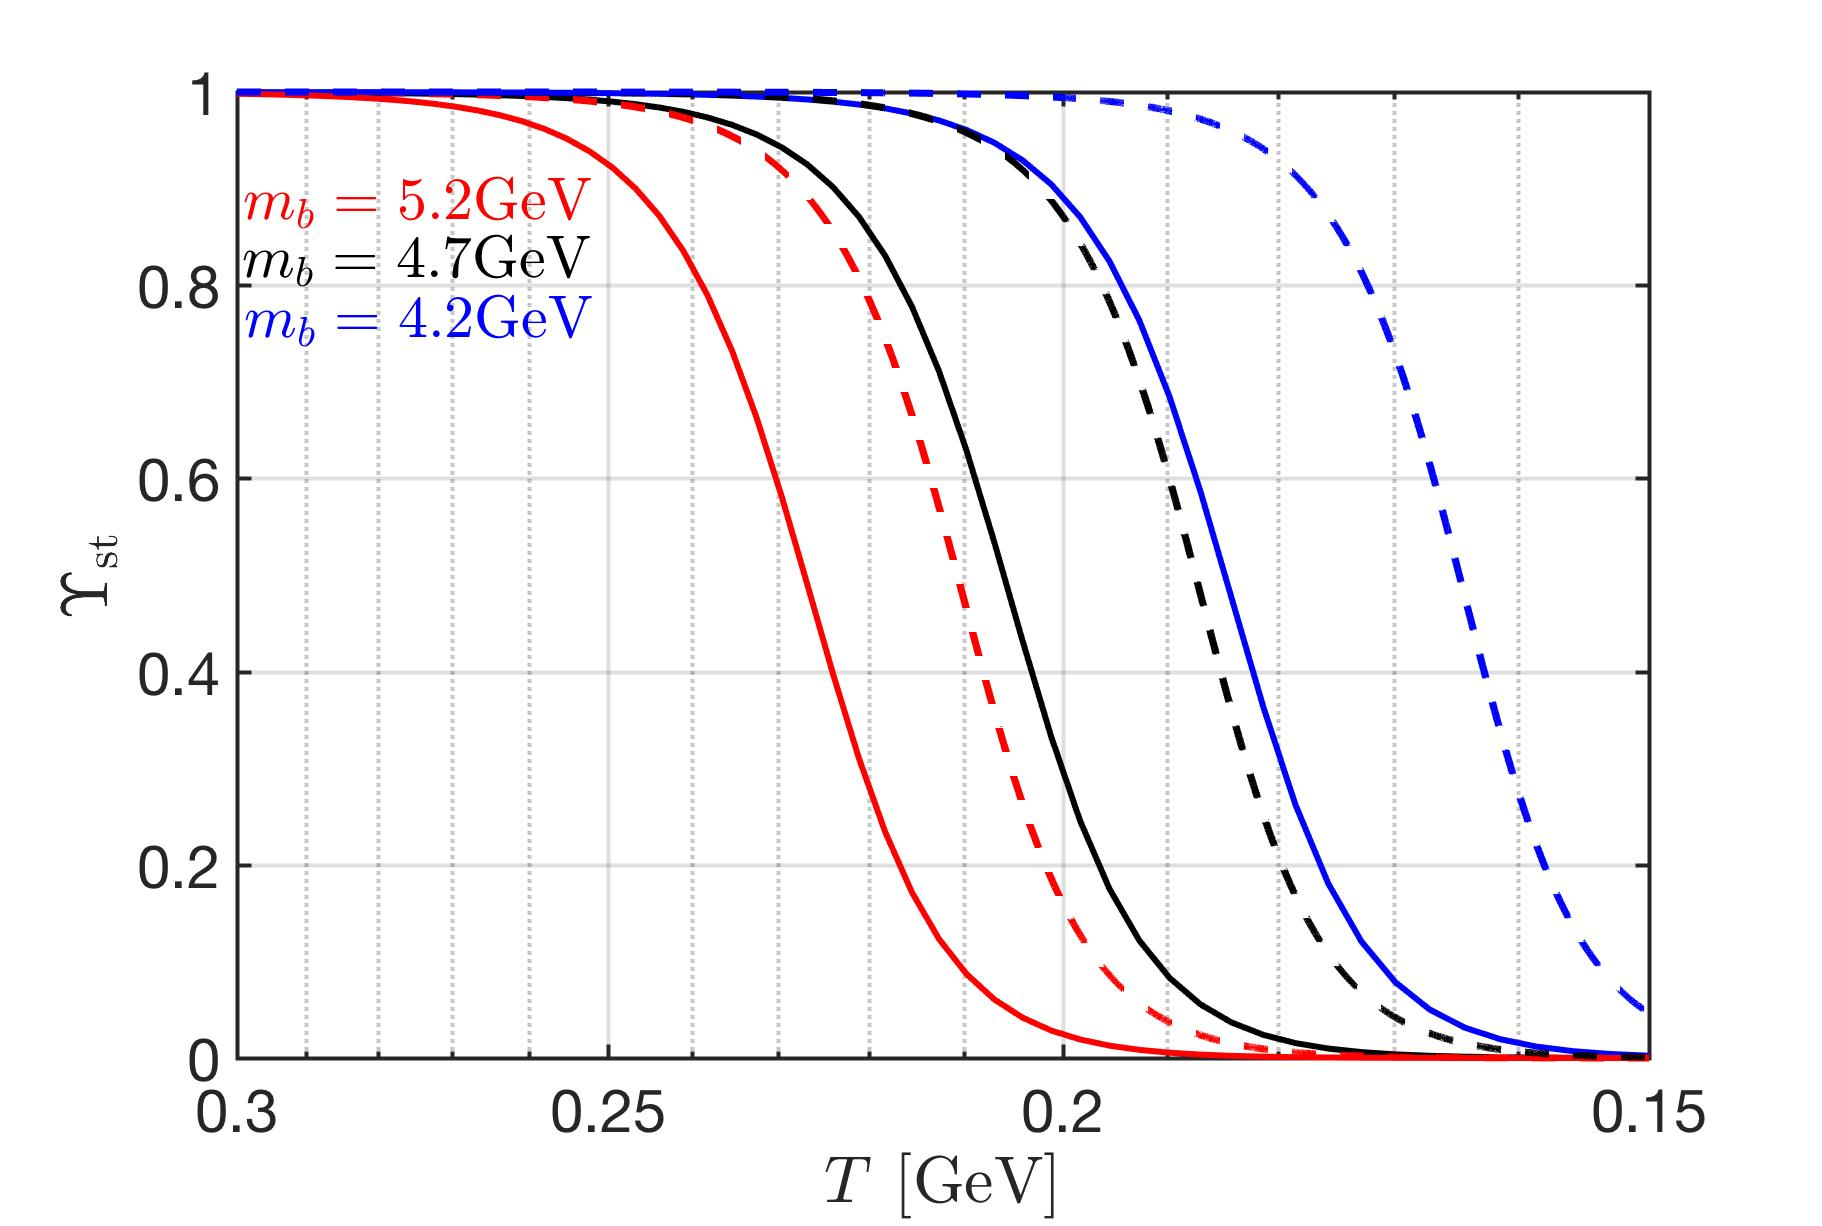
\includegraphics[width=0.9\textwidth]{./plots/BquarkFugacity_tot}}
\caption{\cccite{Rafelski:2023emw}, adapted from thesis of C.T.\,Yang \cite{Yang:2024ret}. Dynamical fugacity of bottom quark as a function of temperature in primordial Universe. Solid line shows bottom quark bound into $B_c$, dashed lines the case of free bottom quark: $m_b=4.2\,\mathrm{GeV}$ (blue), $m_b=4.7\,\mathrm{GeV}$ (black), and $m_b=5.2\,\mathrm{GeV}$ (red)}
\label{fugacity_bc}
\end{figure}
%%%%%%%%%%%%%%%%%%%%%%%%%%%%%%%%%%%%%%%%%

In \rf{fugacity_bc} the fugacity of bottom quark $\Upsilon_{\mathrm{st}}$ as a function of temperature, \req{Fugacity_Sol} is shown around the temperature $T=0.3\,\mathrm{GeV}>T>0.15\,\mathrm{GeV}$ for different masses of bottom quarks. In all cases we see prolonged non-equilibrium, this happens since the decay and reformation rates of bottom quarks are comparable to each other as we have noted in \rf{ReactionTime} where both lines cross. One of the key results shown in \rf{fugacity_bc} is that the smaller mass of bottom quark slows the strong interaction formation rate to the value of weak interaction decays just near the phase transformation of QGP to HG phase. Finally, the stationary fugacity corresponds to the reversible reactions in the stationary Universe. In this case, there is no arrow in time for bottom quark because of the detailed balance.

We now consider non-stationary correction in expanding Universe allowing for the Universe  expanding and thus temperature being a function of time. This leads to non-stationary correction related to time dependent fugacity in the expanding Universe. 

In general, the fugacity of bottom quark can be written as 
\begin{align}\label{Nonstationary_sol}
&\Upsilon_b=\Upsilon_{\mathrm{st}}+\Upsilon^{\mathrm{non}}_{\mathrm{st}}=\Upsilon_\mathrm{st}\left(1+x\right),\quad x\equiv{\Upsilon_\mathrm{st}^{\mathrm{non}}}/{\Upsilon_\mathrm{st}},
\end{align}
where the variable $x$ corresponds to the correction due to non-stationary Universe. Substituting the general solution \req{Nonstationary_sol} into differential equation \req{Fugacity_Eq0}, we obtain
\begin{align}\label{Nonstationary_eq}
\frac{dx}{dt}=-x^2\frac{\Upsilon_\mathrm{st}}{\tau_{source}}&-x\left[\frac{1}{\tau_{eff}}+3H-\frac{1}{\tau_T}\right]-\left[\frac{d\ln\Upsilon_\mathrm{st}}{dt}+3H-\frac{1}{\tau_T}\right],
\end{align}
where the effective relaxation time $1/\tau_{eff}$ is defined as
\begin{align}
\frac{1}{\tau_{eff}}\equiv\left[\frac{2\Upsilon_\mathrm{st}}{\tau_{source}}+\frac{1}{\tau_{decay}}+\frac{d\ln\Upsilon_\mathrm{st}}{dt}\right].
\end{align}

%%%%%%%%%%%%%%%%%%%%%%%%%%%%%%
\begin{figure} 
\centerline{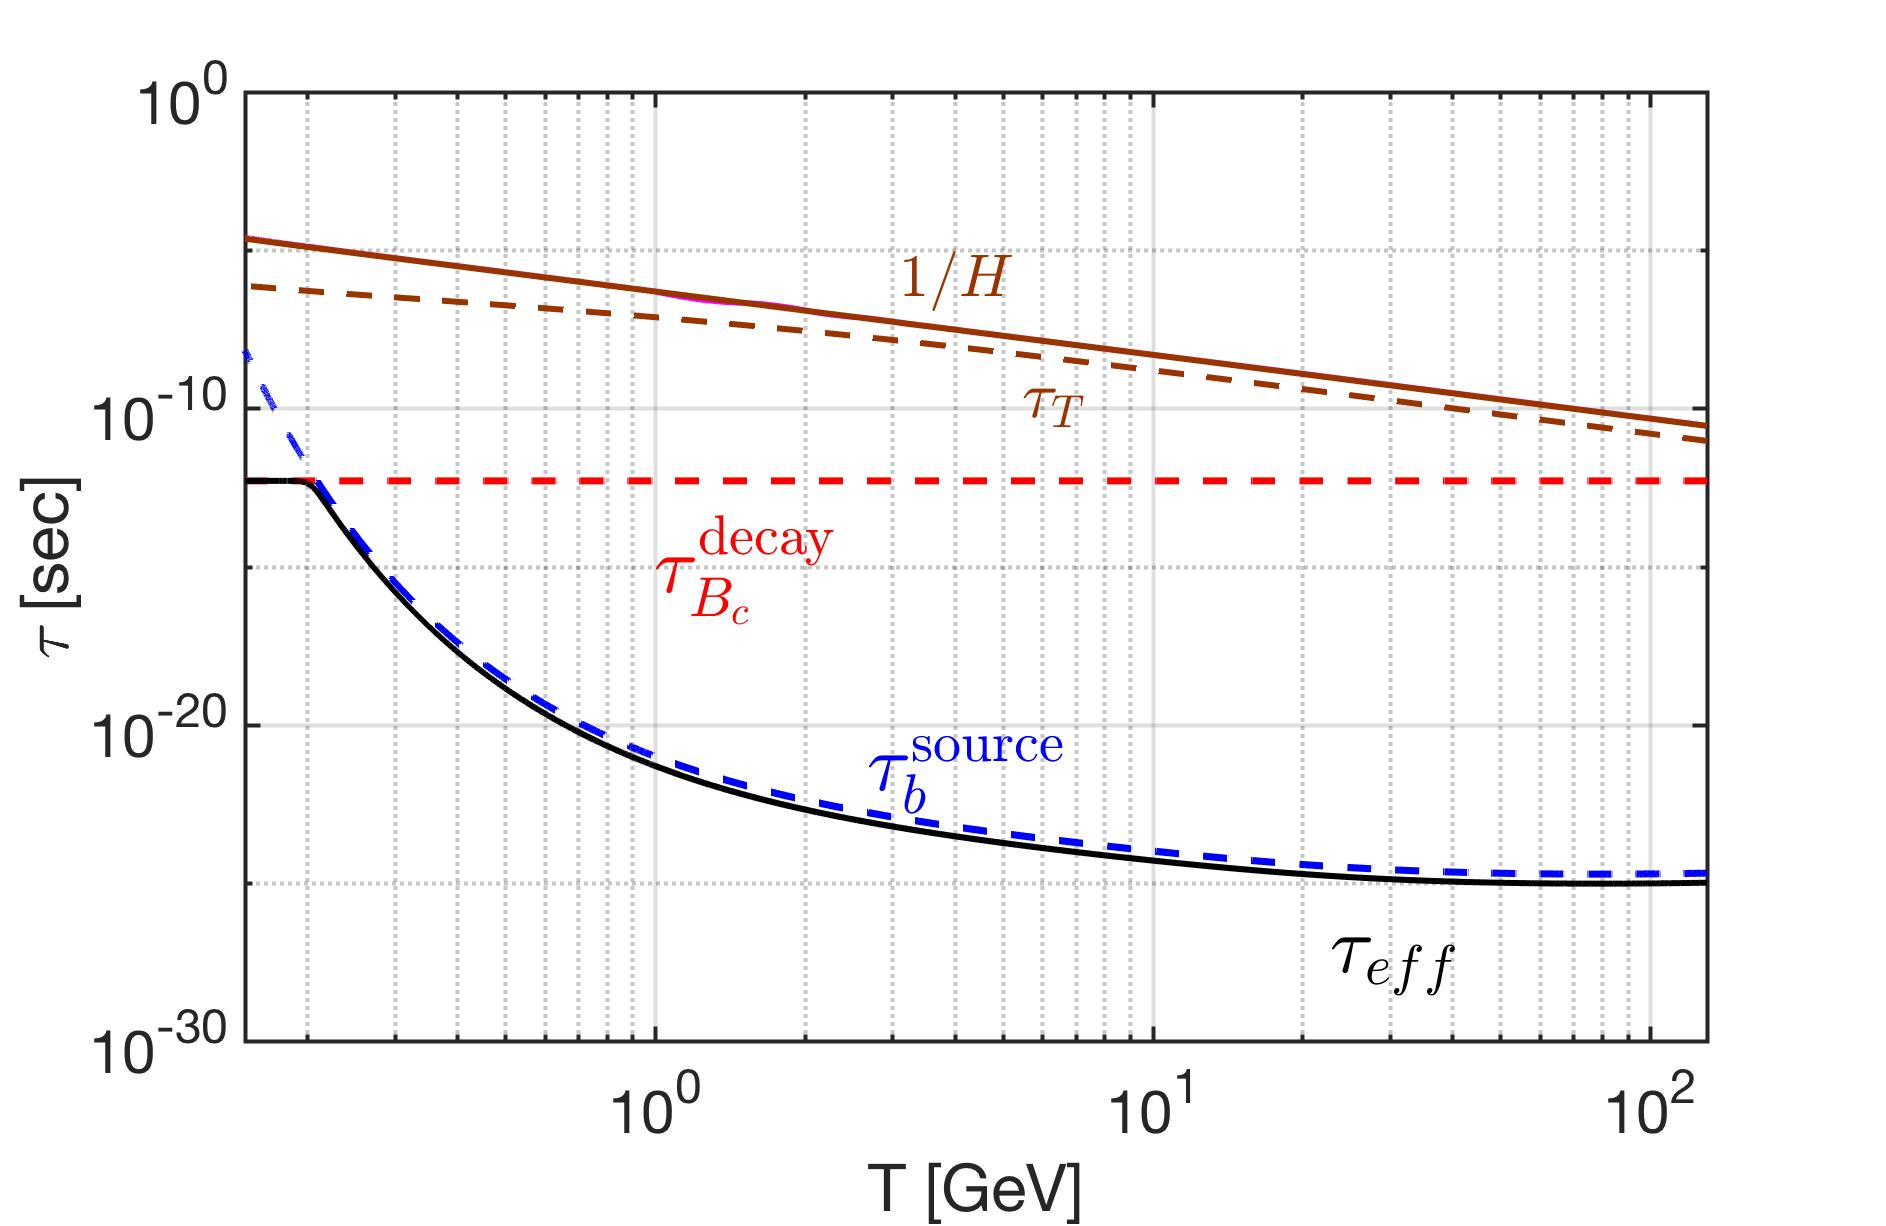
\includegraphics[width=0.9\textwidth]{./plots/Tau_RelaxationTime002}}
\caption{The effective relaxation time $\tau_{eff}$ as a function of temperature in the early Universe for bottom mass $m_b=4.7$\,GeV.  For comparison, we also plot the vacuum lifespan of $B_c$ meson $\tau_{B_c}^{decay}$ (red dashed-line), the relaxation time for bottom production $\tau^b_{source}$ (blue dashed-line), Hubble expansion time $1/H$(brown solid line) and relaxation time for temperature cooling $\tau_T$ (brown dashed-line). Adapted from the thesis of C.T.\,Yang \cite{Yang:2024ret}}
\label{RelaxationTime_eff}
\end{figure}
%%%%%%%%%%%%%%%%%%%%%%%%%%%%%%%%%

In \rf{RelaxationTime_eff} we see that when temperature is near to $T=0.2$ GeV, we have $1/\tau_{eff}\approx10^{7}H$, and $1/\tau_{eff}\approx10^5/\tau_T$. In this case, the last two terms in \req{Nonstationary_eq} compare to $1/\tau_{eff}$ can be neglected, and the differential equation becomes
\begin{align}\label{nonstationary_eq}
\frac{dx}{dt}=-\frac{x^2\,\Upsilon_\mathrm{st}}{\tau_{source}}&-\frac{x}{\tau_{eff}}-\left[\frac{d\ln\Upsilon_\mathrm{st}}{dt}+3H-\frac{1}{\tau_T}\right],
\end{align}


To solve the variable $x$ we consider the case $dx/dt,x^2\ll1$ first, we neglect the terms $dx/dt$ and $x^2$ in \req{nonstationary_eq}  then solve the linear fugacity equation.  We will establish that these approximations are justified by checking the magnitude of the solution. Neglecting terms $dx/dt$ and $x^2$ in \req{nonstationary_eq} we obtain
\begin{align}
x\approx\tau_{eff}\left[\frac{d\ln\Upsilon_\mathrm{st}}{dt}+3H-\frac{1}{\tau_T}\right].
\end{align}
It is convenient to change the variable from time to temperature. For an isentropically-expanding universe, we have
\begin{align}\label{tau_H}
\frac{dt}{dT}=-\frac{\tau^\ast_H}{T},\qquad \tau^\ast_H=\frac{1}{H}\left(1+\frac{T}{3g^s_\ast}\frac{dg^s_\ast}{dT}\right).
\end{align}
In this case, we have
\begin{align}
x=\tau_{eff}\left[\frac{1}{\Upsilon_\mathrm{st}}\frac{d\Upsilon_\mathrm{st}}{dT}\frac{T}{\tau^\ast_H}+3H-\frac{1}{\tau_T}\right].
\end{align}
Finally, we can obtain the nonstationary fugacity by multiplying the fugacity ratio $x$ with $\Upsilon_\mathrm{st}$, giving \index{bottom quark! nonstationary fugacity}
\begin{align}
\Upsilon_{\mathrm{st}}^{\mathrm{non}}
&\approx\left(\frac{\tau_{eff}}{\tau^\ast_H}\right)\left[\frac{d\Upsilon_\mathrm{st}}{dT}T-\Upsilon_{\mathrm{st}}\left(3H\tau^\ast_H-\frac{\tau^\ast_H}{\tau_T}\right)\right].
\end{align}

In \rf{NonFugacity} we plot the nonstationary $\Upsilon^{\mathrm{non}}_\mathrm{st}$ as a function of temperature. The nonstationary fugacity $\Upsilon^{\mathrm{non}}_\mathrm{st}$ follows the behavior of $d\Upsilon_{\mathrm{st}}/dT$, which corresponds to the irreversible process in expanding Universe. In this case, the irreversible nonequilibrium process creates the arrow in time for bottom quark in the Universe. The large value of Hubble time compares to the effective relaxation time suppressing the value of nonstationary fugacity to $\mathcal{O}\sim10^{-7}$, which shows that the neglecting $dx/dt,x^2\ll1$ is a good approximation for solving the non-stationary fugacity in the early Universe.


%%%%%%%%%%%%%%%%%%%%%%%%%%%%%%%%%%%
\begin{figure}[t]
\centerline{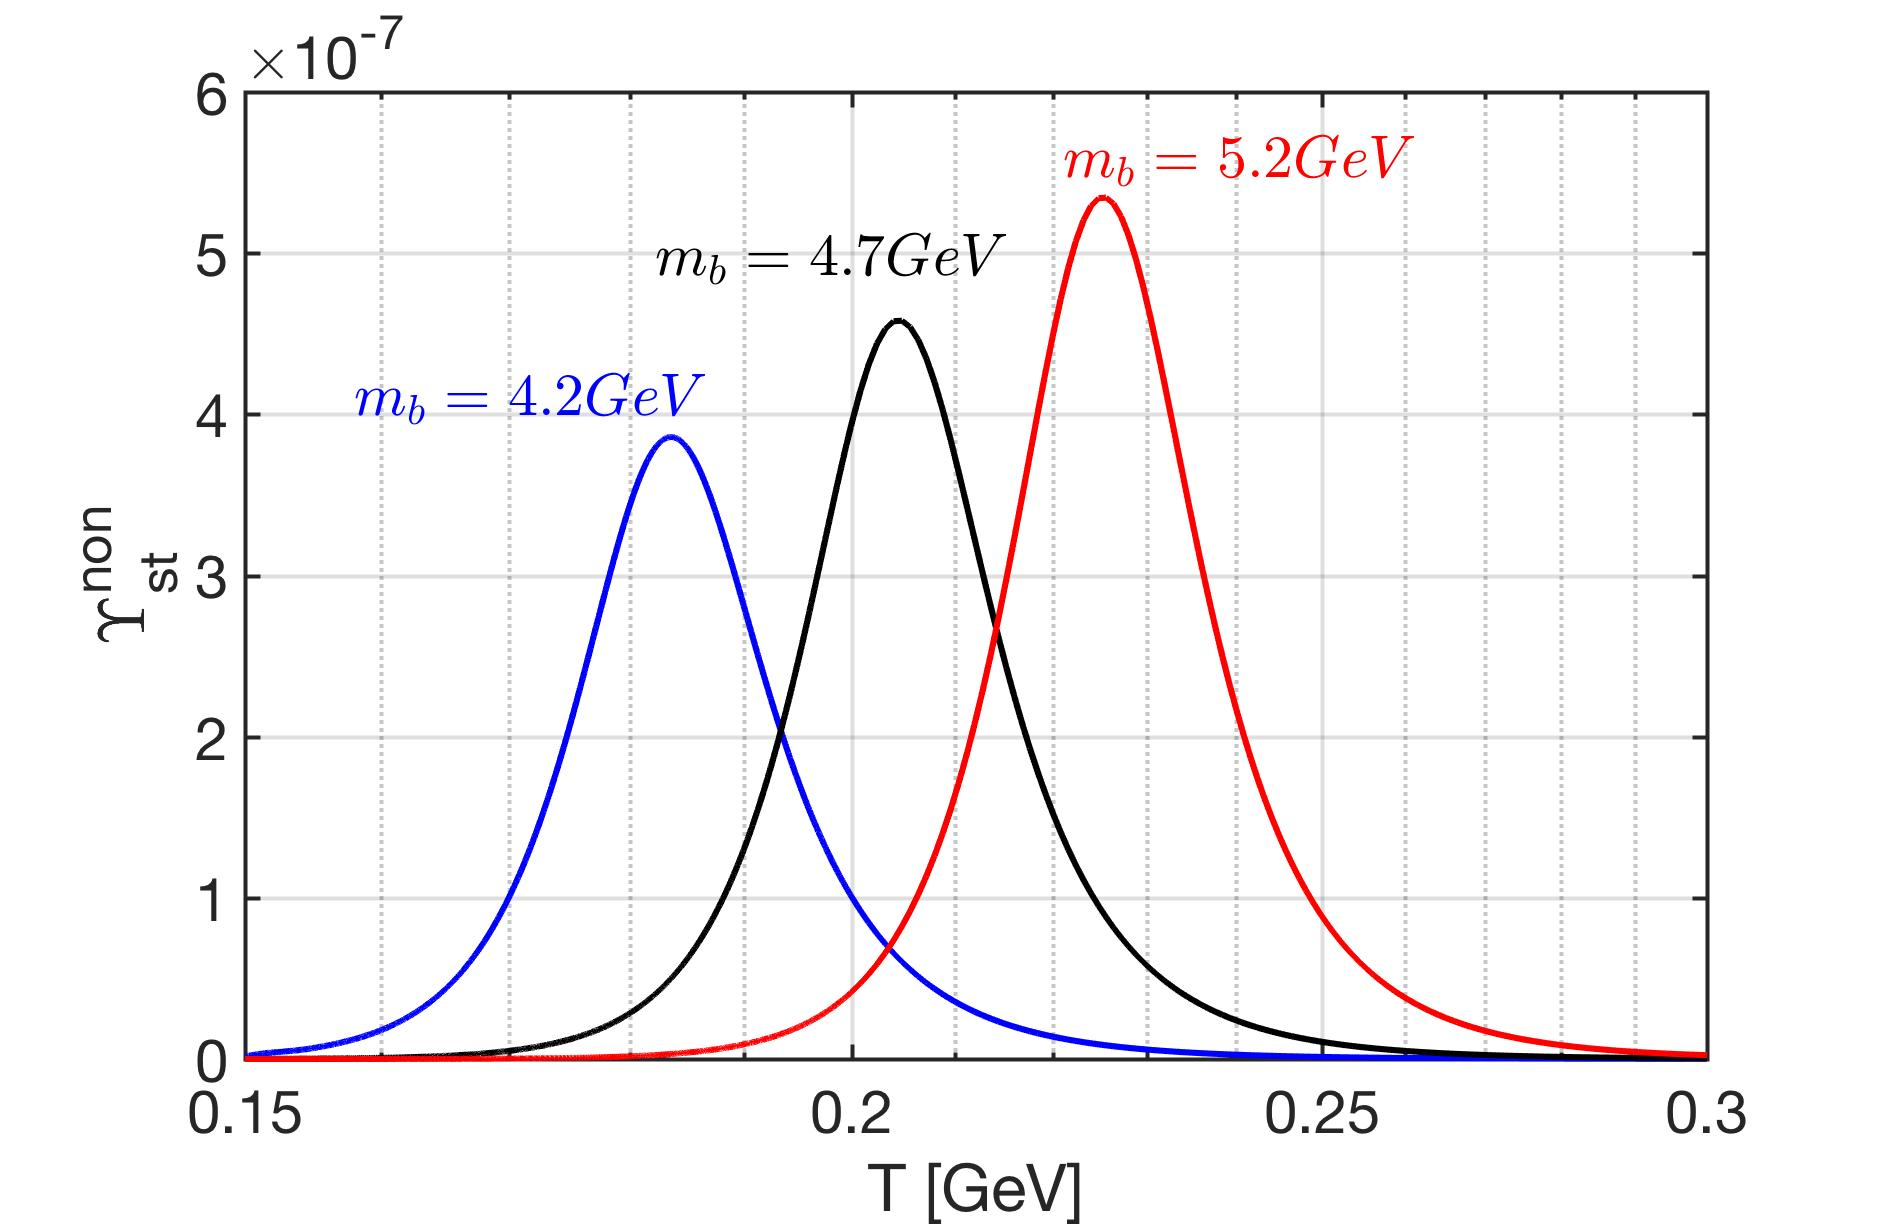
\includegraphics[width=0.9\textwidth]{./plots/NonstationaryFugacity}}
\caption{The non-stationary fugacity $\Upsilon_\mathrm{st}^{\mathrm{non}}$ as a function of temperature in the Universe for different bottom mass $m_b=4.2\,\mathrm{GeV}$ (blue), $m_b=4.7\,\mathrm{GeV}$ (black), and $m_b=5.2\,\mathrm{GeV}$ (red) for the case bottom  quarks bound into $B_c$ mesons. Adapted from the thesis of C.T. Yang \cite{Yang:2024ret}}
\label{NonFugacity}
\end{figure}
%%%%%%%%%%%%%%%%%%%%%%%%%%%%%%%%%%%%%%
 

%%%%%%%%%%%%%%%%%%%%%%%%%%%%%%%%%%
\paragraph{Is there enough bottom flavor to matter?} Considering that FLRW-Universe evolves conserving entropy, and that baryon and lepton number following on the era of matter genesis is conserved, the current day baryon $B$ to entropy $S$, $B/S$-ratio must be achieved during matter genesis. The estimates of present day baryon-to-photon density ratio $\eta$ allows the determination of the present value of baryon per entropy ratio \cite{Rafelski:2019twp,Letessier:2002ony,Fromerth:2002wb,Fromerth:2012fe}:
\begin{align}
\left(\frac{B}{S}\right)_{t_0}\!\!\!\!=\eta\left(\frac{n_\gamma}{\sigma_\gamma+\sigma_\nu}\right)_{\!t_0}\!\!\!\!=(8.69\pm0.05)\!\!\times\!\!10^{-11},
\end{align}
where the subscript $t_0$ denotes the present day value, where $\eta=(6.12\pm0.04)\times10^{-10}$~\cite{ParticleDataGroup:2018ovx} is used in calculation. Here we consider that the Universe today is dominated by photons and free-streaming low mass neutrinos~\cite{Birrell:2012gg}, and $\sigma_\gamma$ and $\sigma_\nu$ are the entropy density for photons and neutrinos, respectively. 
 
In chemical equilibrium the ratio of bottom quark (pair) density $n_b^{th}$ to entropy density $\sigma=S/V$ just above quark-gluon hadronization temperature $T_\mathrm{H}=150\sim160\,\mathrm{MeV}$ is $n_b^{th}/\sigma=10^{-10}\sim10^{-13}$ (see \rf{number_entropy_b002}. By studying the bottom density per entropy near to the hadronization temperature and comparing it to the baryon-per-entropy ratio $B/S$  we found there is sufficient abundance of bottom quarks for the proposed matter genesis mechanism to be relevant.

%%%%%%%%%%%%%%%%%%%%%%%%%%%%%%%%
\paragraph{Example of bottom-catalyzed matter genesis}
Given that the non-equilibrium non-stationary component of bottom flavor arises at relatively low QGP temperature, this Sakharov condition is available around QGP hadronization.   Let us now look back and see how different requirements are fullfilled
%%%%%%%%%%%%%%%%%%%%%%%%%%%%%%%%%%%%
\begin{itemize}
\item
 We have demonstrated non-stationary conditions with absence of detailed balance: The competition between weak interaction decay and the strong interaction gluon fusion process  is responsible for driving the bottom quark departure from the equilibrium in the early Universe near to QGP hadronization condition  around the temperature $T=0.3\sim0.15$ GeV as shown in \rf{fugacity_bc}.  Albeit small there is clear non-stationary component required for baryogenesis, see \rf{NonFugacity}.
%%%%%%%%%%%%%%%%%%%%%%%%%%%%%%%
\item Violation of $CP$ asymmetry were observed in the amplitudes of hadron decay including neutral B-mesons, see for example~\cite{LHCb:2019jta,LHCb:2020vut}. The weak interaction $CP$ violation arises from the components of Cabibbo-Kobayashi-Maskawa (CKM) matrix associated with quark-level transition amplitude and $CP$-violating phase. There is clear coincidence of nonstationary component of bottom yield with  the bottom quark $CP$  violating decays of preformed $\mathrm{B}_x$ meson states, $x=u,d,s,c$~\cite{Karsch:1987pv,Brambilla:2010vq,Aarts:2011sm,Brambilla:2017zei,Bazavov:2018wmo,Offler:2019eij}.  The exploration of the here interesting $CP$ symmetry breaking in B$_c(b\bar c)$ decay is in progress~\cite{Tully:2019ltb,HFLAV:2019otj,ParticleDataGroup:2018ovx}.  % Present measurements of $CP$-violation suggest that the CP asymmetry parameter is around $\delta_{CP}\approx10^{-3}$ ~\cite{ParticleDataGroup:2018ovx}.
\item
We do not know if there is baryon number violating process in which one of the heavy particles, including bottom quark, is participating. However, if such a process were to exist it is likely, considering mass thresholds, that it would be most active in the decays of heaviest standard model particles. It is thus of considerable interst to study in lepton colliders baryon number nonconserving processes at resonance condition. Such a research program will additionally be motivated by our demonstration of an extended period of baryogenesis in the primordial Universe. 
\end{itemize}

%%%%%%%%%%%%%%%%%%%%


 \paragraph{Circular Urca amplification}
 The off equilibrium phenomenon of bottom quark around the temperature range $T=0.3\sim0.15$ GeV can provide the non-chemical equilibrium non-stationary condition for baryogenesis to occur in the primordial-QGP hadronization era. The processes of interest as we saw are small. However there is additional amplifying factor. 
 
 Let us consider the scenario where all bottom quarks are confined within $B_c^\pm$ meson. In this case, the decay of charged mesons in the primordial-QGP can be a source of $CP$ violation. However, it remains uncertain whether the decay of $B_c^\pm$ mesons contributes to baryon violation. Our postulation is as follows: the baryon asymmetry is produced by the bottom quark disappearance via the irreversible decay of $B^\pm_c$ meson during the off-equilibrium process. Once a baryon symmetry exists in universe, it will also produce the asymmetry between leptons and anti-leptons which is similar to the baryon asymmetry by the $L=B$.

The heavy $B_c^\pm$ meson decay into multi-particles in plasma is associated with the irreversible process. This is because after decay the daughter particles can interact with plasma and distribute their energy to other particles and reach equilibrium with the plasma quickly. In this case the  energy required for the inverse reaction to produce $B_c^\pm$ meson is difficult to overcome and therefore we have an irreversible process for multi-particle decay in plasma.


The rapid $B_c^\pm$ decay and bottom reformation speed at picosecond scale assures that there are millions of individual microscopic processes involving bottom quark production and decay before and during the hadronization epoch of QGP. In this case, we have an Urca process for the bottom quark, i.e. a cycling reaction that produces the bottom quark which subsequently  disappears via the $B_c^\pm$ meson decay. 

The Urca process is a fundamental physical process  and has been studying the realms of in astrophysics and nuclear physics. In our case, for bottom quark as a example: at low temperature, the number of bottom quark cycling can be estimated as
\begin{align}
\left.\mathrm{C_{cycle}}\right|_{T=0.2\mathrm{GeV}}=\frac{\tau_H}{\tau_{B_c}}\approx2\times10^7,
\end{align}
where the lifespan of $B_c^\pm$ is  $\tau_{\mathrm{B}_c}\approx0.51\times10^{-12}\,\mathrm{sec}$ and at temperature $T=0.2$ GeV the Hubble time is $\tau_H=1/H=1.272\times10^{-5}$ sec. The Urca process plays a significant role by potentially amplifying any small and currently unobserved violation of baryon number associated with the bottom quark. The small baryon asymmetry is enhanced by the Urca-like process with cycling ${\tau^\ast_H}/{\tau_\ast}$ in the early Universe.
This amplification would be crucial for achieving the required strength for today's observation. 

%%%%%%%%%%%%%%%%%%%%%%%%%%%%%%%%%%%%%%%%%%%%%%%%
\subsection{Hadronization and strangeness abundance in cosmic plasma}
\label{Strangeness}
%%%%%%%%%%%%%%%%%%%%%%%%%%%%%%%%%%
\paragraph{Hadronization of primordial QGP}
As the Universe expanded and cooled down to the  QGP Hagedorn temperature $T_H\approx150$ MeV, the primordial QGP underwent a phase transformation called hadronization. This transition resulted in the confinement of the strong force, causing quarks and gluons to combine and form matter 
and antimatter. After hadronization, one may think the relatively short lived massive hadrons decay rapidly and disappear from the Universe. However, the most abundant hadrons, pions $\pi(q\bar q)$, can be produced via their inverse decay process $\gamma\gamma\rightarrow\pi^0$ and retain their chemical equilibrium until temperature $T=3\sim5$ MeV~\cite{Kuznetsova:2008jt}. 

Following the idea and the framework presented by~\cite{Kuznetsova:2008jt}, we investigate the strange particle composition of the expanding early Universe in the epoch $150\,\mathrm{MeV}\ge T\ge 10$\,MeV, and examine the freeze-out temperature for strangeness-producing  by comparing the relevant reaction rates to the Hubble expansion rate. We show that strangeness is kept in equilibrium via weak, electromagnetic, and strong interactions in the early Universe until $T\approx13$ MeV.

At first we explore the Universe composition assuming both kinetic and particle abundance equilibrium (chemical equilibrium) by considering the charge neutrality and prescribed conserved baryon-per-entropy-ratio ${(n_B-n_{\overline{B}})}/{\sigma}$ to determine the baryon chemical potential $\mu_B$~\cite{Fromerth:2012fe,Rafelski:2013yka}. With the chemical potential as a function of temperature, we can obtain the particle number densities for different species and study their composition in the early Universe.

We improve the prior work~\cite{Fromerth:2012fe} by considering the conserved entropy per baryon ratio with conservation of strangeness in the early Universe. To study the baryon and strange quark chemical potential, it is convenient to introduce the chemical fugacity for strangeness $\lambda_s$ and quark $\lambda_q$ as follows:\index{baryon chemical potential}
\begin{align}
\lambda_s=\exp(\mu_s/T)\,\quad \lambda_q=\exp(\mu_B/3T),
\end{align}
where $\mu_s$ and $\mu_B$ are the chemical potential of strangeness and baryon, respectively. For the quark fagucity $\lambda_q$, we divide the chemical potential of baryons by 3 as an approximation for quark chemical potential. 

Imposing the conservation of strangeness  
$\langle s-\bar s \rangle=0$, we have, when the baryon chemical potential does not vanish the chemical potential of strangeness in the early Universe satisfying (see Section 11.5 in \,\cite{Letessier:2002ony})\index{strange quark! chemical potential}
\begin{align}\label{museq}
\lambda_s=\lambda_q\sqrt{\frac{F_K+\lambda^{-3}_q\,F_Y}{F_K+\lambda^3_q\,F_Y}}.
\end{align}
where we employ the phase-space function $F_i$ for sets of nucleon $N$, kaon $K$, and hyperon $Y$ particles defined as (see \cite{Letessier:2002ony}, Section 11.4):
\begin{align}
&F_N=\sum_{N_i}\,g_{N_i}W(m_{N_i}/T)\;, \quad N_i=n, p, \Delta(1232),\\
&F_K=\sum_{K_i}\,g_{K_i}W(m_{K_i}/T)\;, \quad K_i=K^0, \overline{K^0}, K^\pm, K^\ast(892),\\
&F_Y=\sum_{Y_i}\,g_{Y_i}W(m_{Y_i}/T)\;, \quad Y_i=\Lambda, \Sigma^0,\Sigma^\pm, \Sigma(1385),
\end{align}
where $g_{N_i,K_i,Y_i}$ are the degenerate factors, $W(x)=x^2K_2(x)$ with $K_2$ is the modified Bessel functions of integer order "$2$".  

Considering the Boltzmann approximation for the massive particle number density we have
\begin{align}
\label{Density_N}
&n_N=\frac{T^3}{2\pi^2}\lambda_q^3F_N,\quad\qquad\qquad n_{\overline N}=\frac{T^3}{2\pi^2}\lambda^{-3}_qF_N,\\
\label{Density_K}
&n_K=\frac{T^3}{2\pi^2}\left(\lambda_s\lambda_q^{-1}\right)F_K,\,\qquad n_{\overline{K}}=\frac{T^3}{2\pi^2}\left(\lambda_s^{-1}\lambda_q\right)F_K,\\
\label{Density_Y}
&n_Y=\frac{T^3}{2\pi^2}\left(\lambda_q^2\lambda_s\right)F_Y,\quad\qquad n_{\overline Y}=\frac{T^3}{2\pi^2}\left(\lambda^{-2}_q\lambda_s^{-1}\right)F_Y.
\end{align}
In this case, the net baryon density in the early Universe with temperature range $150\,\mathrm{MeV}> T>10$\,MeV can be written as 
\begin{align}
\frac{\left(n_B-n_{\overline{B}}\right)}{\sigma}&=\frac{1}{\sigma}\left[\left(n_p-n_{\overline{p}}\right)+\left(n_n-n_{\overline{n}}\right)+\left(n_Y-n_{\overline{Y}}\right)\right]\notag\\
&=\frac{T^3}{2\pi^2\,\sigma}\left[\left(\lambda_q^3-\lambda^{-3}_q\right)F_N+\left(\lambda_q^2\lambda_s-\lambda^{-2}_q\lambda_s^{-1}\right)F_Y\right]\notag\\
&=\frac{T^3}{2\pi^2\sigma}\left(\lambda_q^3-\lambda_q^{-3}\right)F_N\left[1+\frac{\lambda_s}{\lambda_q}\left(\frac{\lambda_q^3-\lambda^{-1}_q\lambda_s^{-2}}{\lambda^3_q-\lambda^{-3}_q}\right)\,\frac{F_Y}{F_N}\right]\notag\\
&\approx\frac{T^3}{2\pi^2\sigma}\left(\lambda_q^3-\lambda_q^{-3}\right)F_N\left[1+\frac{\lambda_s}{\lambda_q}\,\frac{F_Y}{F_N}\right],
\end{align}
where we can neglect the term $F_Y/F_K$ in the expansion of Eq.(\ref{museq}) in our temperature range. 

Introducing the strangeness $\langle s-\bar s\rangle=0$ constraint and using the entropy density in early universe, the explicit relation for baryon to entropy ratio becomes
\begin{align}\label{muBeq}
\frac{n_B-n_{\overline{B}}}{\sigma}&=\frac{45}{2\pi^4g^s_\ast}\sinh\left[\frac{\mu_B}{T}\right]F_N\times\left[1+\frac{F_Y}{F_N}\sqrt{\frac{1+e^{-\mu_B/T}\,F_Y/F_K}{1+e^{\mu_B/T}\,F_Y/F_K}}\right].
\end{align}
Governing Eq.\,(\ref{muBeq}) is the present-day baryon-per-entropy-ratio, and we obtain the value 
\begin{align}\label{BdS}
\frac{n_B-n_{\overline{B}}}{\sigma}= \left.\frac{n_B-n_{\overline{B}}}{ \sigma}\right|_{t_0}=(0.865\pm0.008)\times10^{-10} \;.
\end{align}

For a detailed evaluation method we refer to this earlier work now using a baryon-to-photon ratio~\cite{ParticleDataGroup:2018ovx}: $\left(n_B-n_{\overline{B}}\right)/n_\gamma= (0.609\pm0.06)\times10^{-9}$, as well as the entropy per particle for a massless boson $\sigma/n|_\mathrm{boson}\approx 3.60$ and a massless fermion $\sigma/n|_\mathrm{fermion}\approx 4.20$. 

%%%%%%%%%%%%%%%%%%%%%%%%
\begin{figure} 
\centerline{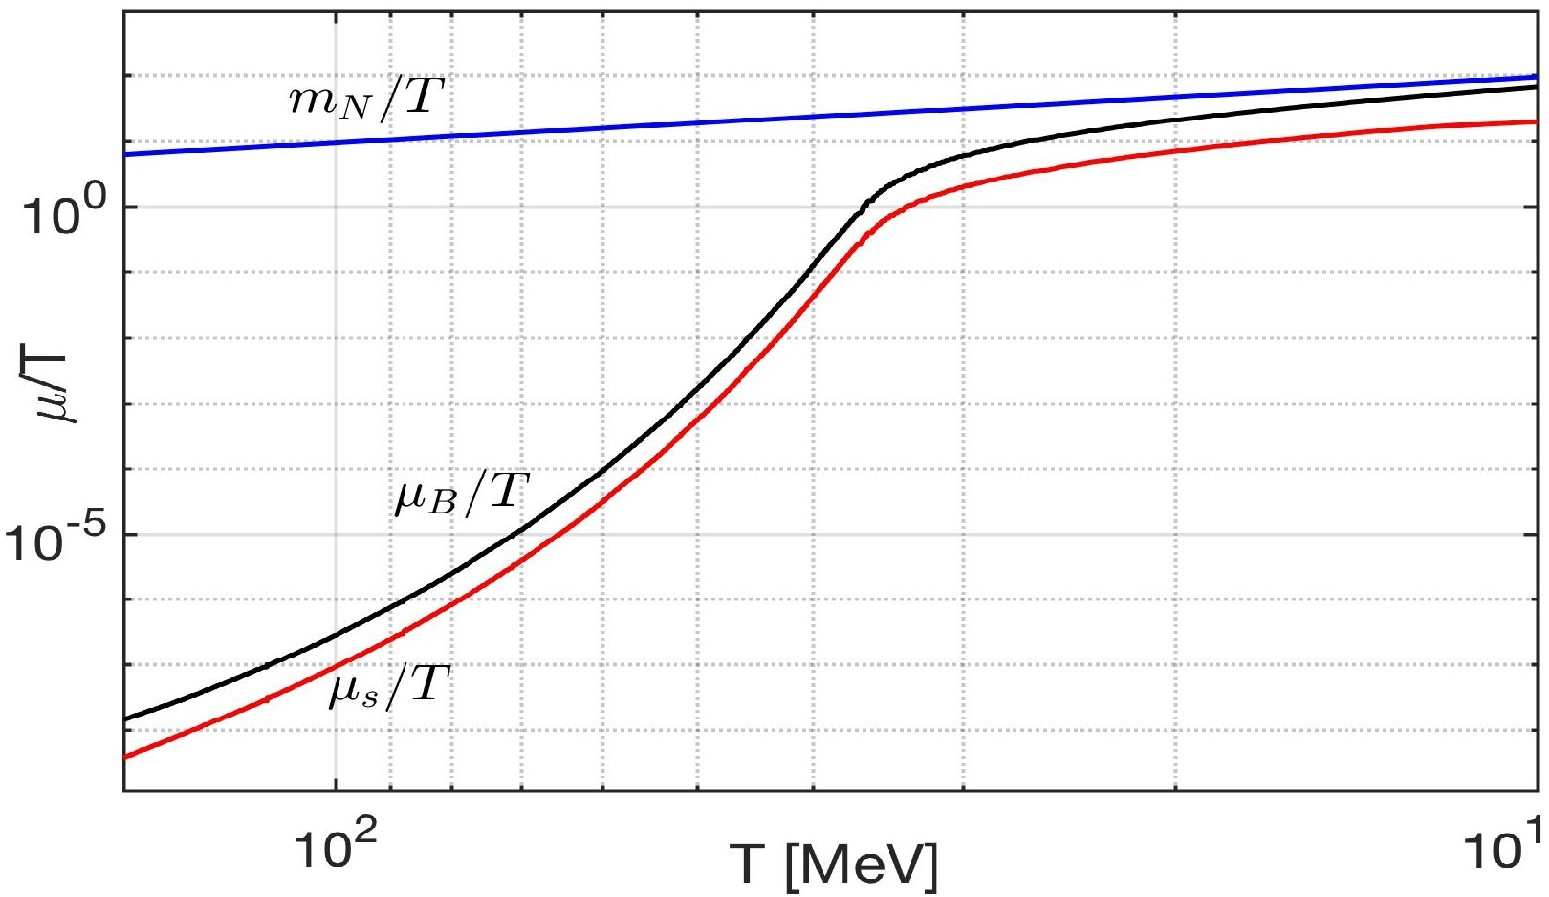
\includegraphics[width=0.9\textwidth]{./plots/New_Chemical_Potential_C.jpg}}
\caption{\cccite{Yang:2021bko}, adapted from thesis of C.T.Yang \cite{Yang:2024ret}. The chemical potential of baryon $\mu_B/T$ and strangeness $\mu_s/T$ as a function of temperature $150\,\mathrm{MeV}> T>10\,\mathrm{MeV}$ in the early Universe; for comparison we show $m_N/T $ with $m_N=938.92$\,MeV, the average nucleon mass}
\label{ChemPotFig} 
\end{figure}
%%%%%%%%%%%%%%%%%%%%%%%%%%%%%%

%%%%%%%%%%%%%%%%%%%%%%%%%%%%%%%%%%%%%%%
\begin{figure} 
\centerline{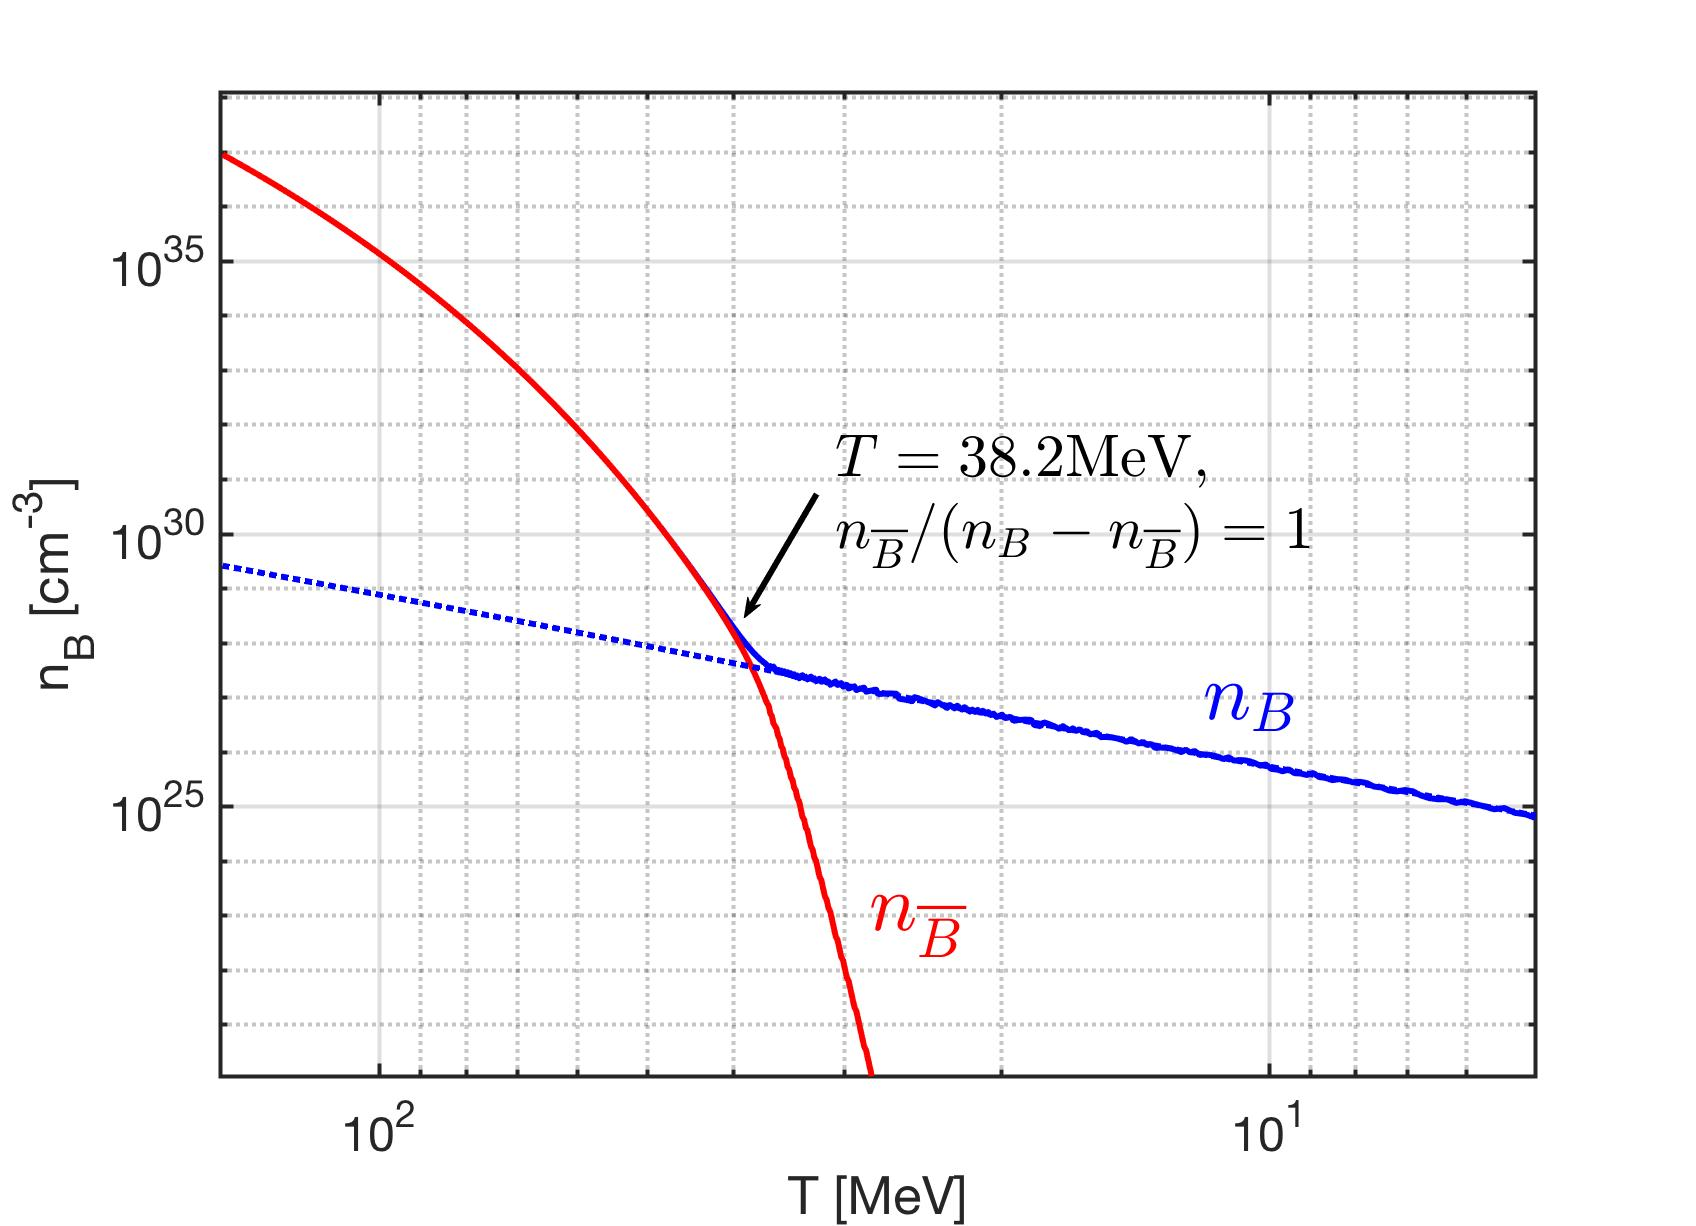
\includegraphics[width=0.9\textwidth]{./plots/Baryon_Antibaryon_cm.jpg}}
\caption{\cccite{Rafelski:2023emw}, adapted from thesis of C.T.Yang \cite{Yang:2024ret}. The baryon (blue solid line) and antibaryon (red solid line) number density as a function of temperature in the range $150\,\mathrm{MeV}>T>5\,\mathrm{MeV}$. The blue dotted line is the extrapolated value for baryon density. The temperature $T=38.2\,\mathrm{MeV}$ is denoted when the ratio $n_{\overline B}/(n_B-n_{\overline B})=1$ which defines the condition where antibaryons disappear from the Universe}
\label{Baryon_fig}
\end{figure}
%%%%%%%%%%%%%%%%%%%%%%%%%%%%%%%%%%%%%%%


We solve  \req{museq}) and \req{muBeq} numerically to obtain baryon and strangeness chemical potentials as a function of temperature in  \rf{ChemPotFig}. The chemical potential changes dramatically in the temperature window $50\,\mathrm{MeV}\le T\le 30$\,MeV, its behavior describing the process of antibaryon disappearance. Substituting the chemical potential $\lambda_q$ and $\lambda_s$ into particle density \req{Density_N}, \req{Density_K}, and \req{Density_Y}, we can obtain the particle number densities for different species as a function of temperature.

In \rf{Baryon_fig} we plot the number density of baryon and antibaryon as a function of temperature. We consider that when the  $n_{\overline B}\ll(n_B-n_{\overline B})$ the anitbaryons density is sufficient low and disappear from the Universe inventory quickly. To determine the temperature where antibaryons is sufficient law in the Universe inventory we defined the condition when the ratio $n_{\overline B}/(n_B-n_{\overline B})=1$. This condition is reached in an expanding Universe at $T=38.2$\,MeV, which is in agreement with the qualitative result in \cite{Kolb:1990vq}. After this temperature, the net baryon density dilutes with a residual co-moving conserved quantity determined by the observed baryon asymmetry.

%%%%%%%%%%%%%%%%%%%%%%%%%%%%
\begin{figure}  
\centerline{
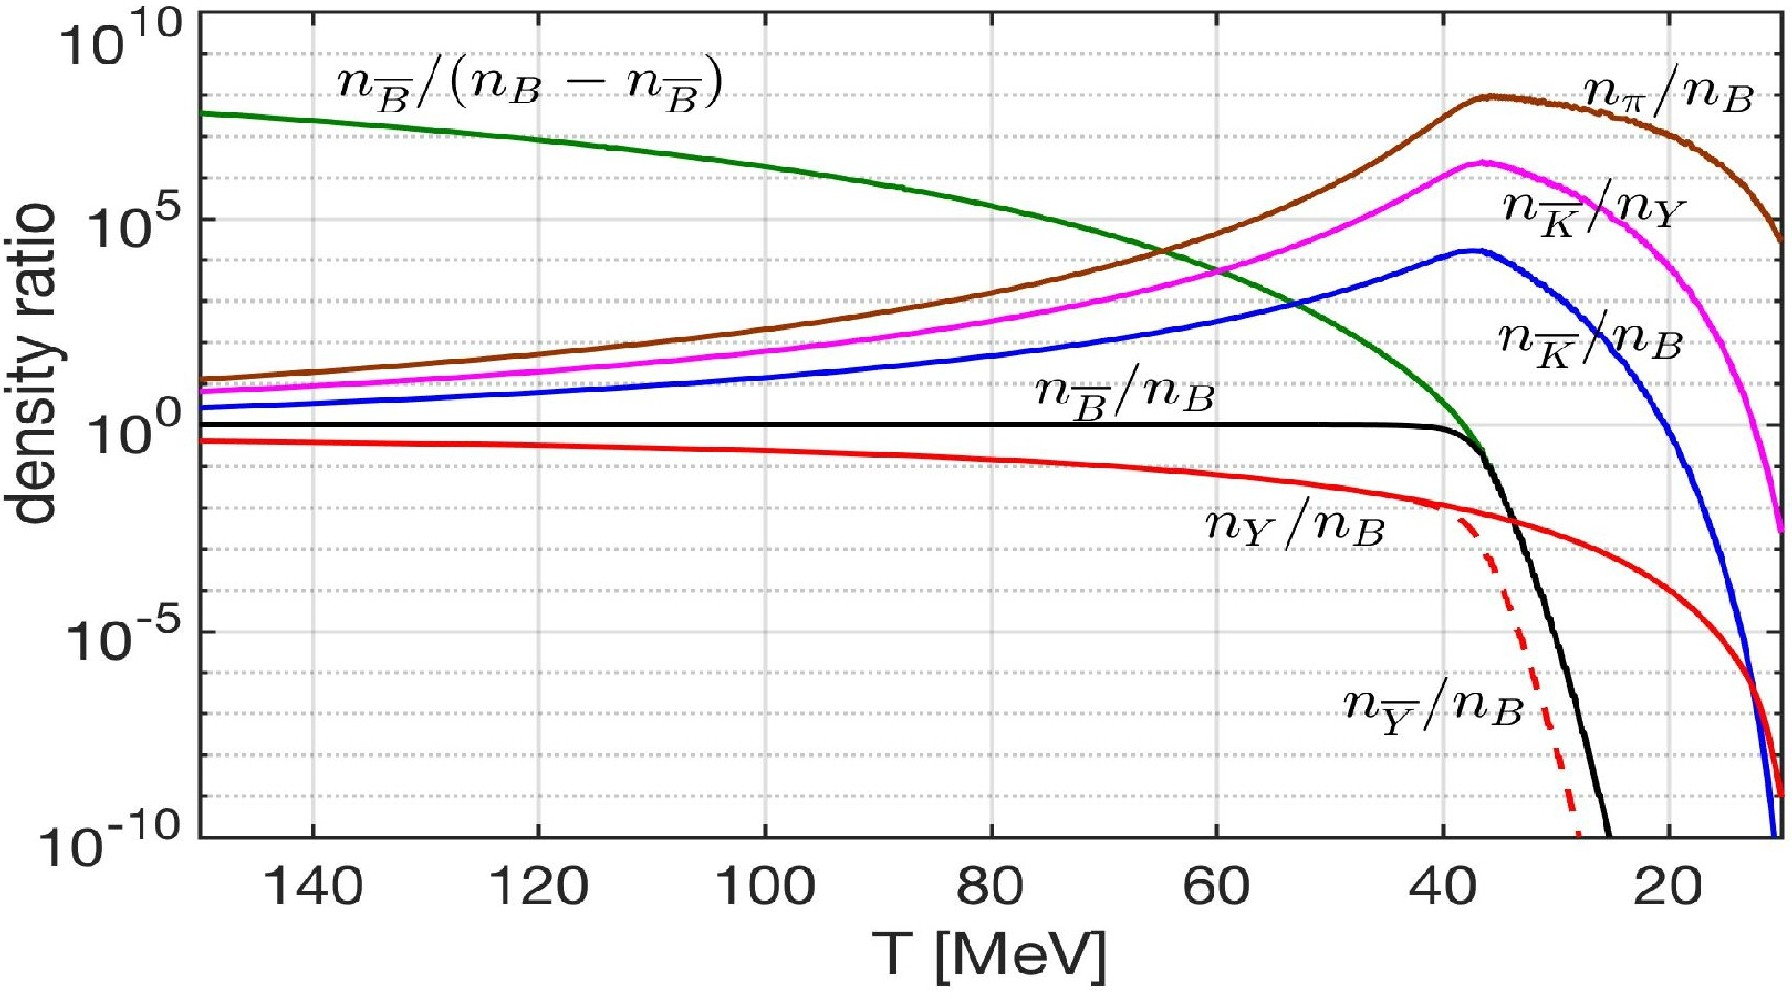
\includegraphics[width=0.9\textwidth]{./plots/Meson_Baryon_density_ratio_C.jpg}}
\caption{\cccite{Rafelski:2023emw}, adapted from Ref.~\cite{Yang:2021bko} and thesis of C.T.Yang \cite{Yang:2024ret}. Ratios of hadronic particle number densities as a function of temperature $150\,\mathrm{MeV}> T>10\,\mathrm{MeV}$ in the early Universe, with baryon $B$ yields: pions $\pi$ (brown line), kaons $K( q\bar s)$ (blue), antibaryon $\overline B$ (black), hyperon $Y$ (red) and anti-hyperons $\overline Y$ (dashed red). Also shown $\overline K/Y$(purple)}
\label{EquilibPartRatiosFig} 
\end{figure}
%%%%%%%%%%%%%%%%%%%%%%%%%%%

In \rf{EquilibPartRatiosFig} we show examples of particle abundance ratios of interest\index{hadron density}. %Considering $n_Y/n_B$ we see that hyperons $Y(sqq)$ remain a noticeable 1\% component in baryon yield through this domain of antibaryon decoupling.
Pions $\pi(q\bar q)$ are the most abundant hadrons $n_\pi/n_B\gg1$, because of their low mass and the reaction $\gamma\gamma\rightarrow\pi^0$, which assures chemical yield equilibrium~\cite{Kuznetsova:2008jt}. For $150\,\mathrm{MeV}>T>20.8\,\mathrm{MeV}$, we see the ratio $n_{{\overline K}(\bar q s)}/n_B\gg1$, which implies pair abundance of strangeness is more abundant than baryons, and is dominantly present in mesons, since $n_{\overline K}/n_Y\gg1$. 

For $20.8\,\mathrm{MeV}>T$, the baryon becomes dominant $n_{\overline K}/n_B<1$, which implies that the strange meson is embedded in a large background of baryons, and the exchange reaction $\overline{K}+N\rightarrow \Lambda+\pi$ can re-equilibrate kaons and hyperons in the temperature range; therefore strangeness symmetry $s=\bar s$ is maintained. For $12.9\,\mathrm{MeV}>T$ we have $n_Y/n_B>n_{\overline K}/n_B$, now the still existent tiny abundance of strangeness is found predominantly in hyperons.

%%%%%%%%%%%%%%%%%%%%%%%%%%%%%%%%%
\paragraph{Strangeness freeze-out}
We now explore strangeness in hadronic `normal matter' particles during and after the hadronization process of QGP. To study the strangness population we will need to explore a large number of reactions, going well beyond the relative simplicity of the QGP phase of  matter. 

Let us first consider an unstable strange particle $S$ decaying into two particles $1$ and $2$, which themselves have no strangeness content. In a dense and high-temperature plasma with particles $1$ and $2$ in thermal equilibrium, the inverse reaction populates the system with particle $S$. This is written schematically as
\begin{align}
 S\Longleftrightarrow1+2,\qquad \mathrm{Example}: K^0\Longleftrightarrow\pi+\pi\,.
\end{align}
The natural decay of the daughter particles provides the intrinsic strength of the inverse strangeness production reaction rate. As long as both decay and production reactions are possible, particle $S$ abundance remains in thermal equilibrium; as already discussed this balance between production and decay rates is the `detailed balance'.

Once the primordial Universe expansion rate $1/H$ overwhelms the strongly temperature dependent back-reaction and the back reaction freeze-out, then the decay $S\rightarrow 1+2$ occurs out of balance and particle $S$ disappears rather rapidly from the inventory. 

Second on our list are the two-on-two strangeness producing reactions. These have a significantly higher strangeness production reaction threshold, thus especially near to strangeness decoupling their influence is negligible. Such reactions are more important near the QGP hadronization temperature $T_H\simeq 150$\,MeV, and they characterize strangeness exchange reactions such as $\mathrm{K}+N\leftrightarrow \Lambda+\pi$, (see Chapter 18 in \cite{Letessier:2002ony}).

In \rf{Strangeness_map2} we show reactions relevant to strangeness evolution in the considered Universe evolution epoch $150\,\mathrm{MeV}\ge T\ge 10$\,MeV  and their pertinent reaction strength. 
%%%%%%%%%%%%%%%%%%%%%%%%%%%%%%%%%%%%%%%
\begin{figure}  
\centerline{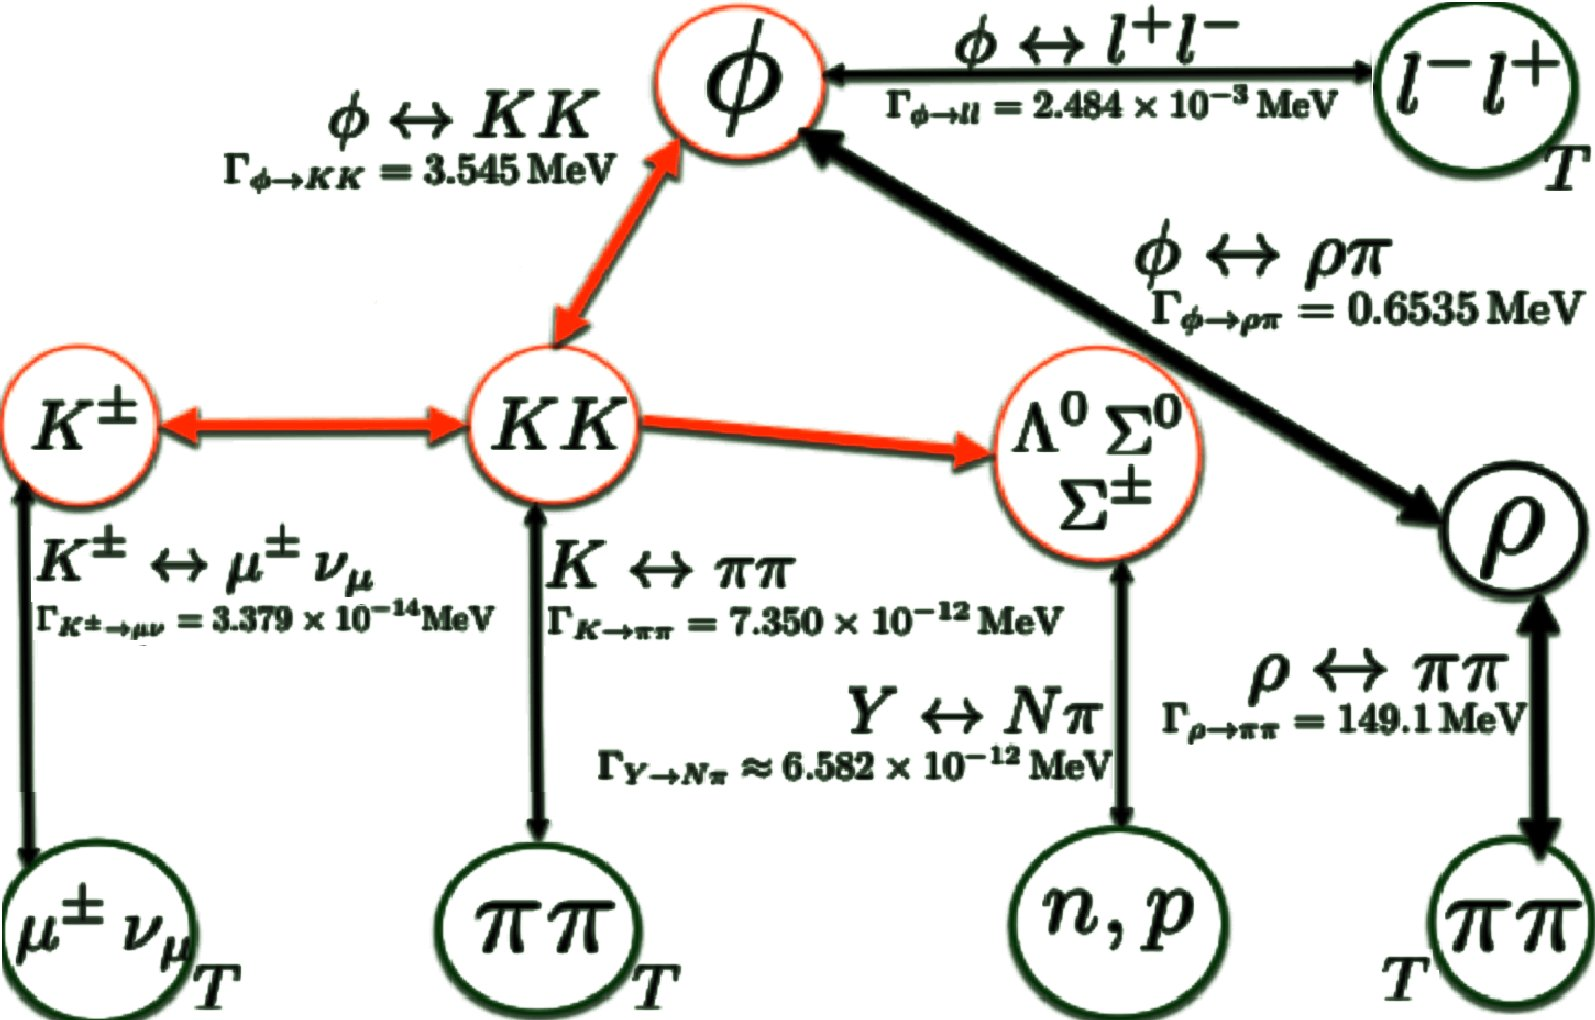
\includegraphics[width=0.9\linewidth]{./plots/Strangeness002_newJ.jpg}}
\caption{\cccite{Rafelski:2023emw}, adapted from Ref.~\cite{Yang:2021bko} and thesis of C.T.Yang \cite{Yang:2024ret}. The strangeness abundance changing reactions in the primordial Universe. The red circles show strangeness carrying hadronic particles; red thick lines denote effectively instantaneous reactions. Black thick lines show relatively strong hadronic reactions. The reaction rates required to describe  strangeness time evolution are shown in \cite{Rafelski:2020ajx} 
}
\label{Strangeness_map2} 
\end{figure}
%%%%%%%%%%%%%%%%%%%%%%%%%%%%%%%%%%%%
Specifically:
\begin{itemize}
\item
We study strange quark abundance in baryons and mesons, considering both open and hidden strangeness (hidden: $s\bar s$-content). Important source reactions are $l^-+l^+\rightarrow\phi$, $\rho+\pi\rightarrow\phi$, $\pi+\pi\rightarrow K_\mathrm{S}$, $\Lambda \leftrightarrow \pi+ N$, and $\mu^\pm+\nu\rightarrow K^\pm$. 
\item
Muons and pions are coupled through electromagnetic reactions $\mu^++\mu^-\leftrightarrow\gamma+\gamma$ and $\pi\leftrightarrow\gamma+\gamma$ to the photon background and retain their chemical equilibrium until the temperature $T =4$\, MeV and $T=5$\,MeV, respectively~\cite{Rafelski:2021aey,Kuznetsova:2008jt}. The large $\phi\leftrightarrow K+K$ rate assures $\phi$ and $K$ are in relative chemical equilibrium.
\end{itemize}
In order to determine where exactly strangeness disappears from the Universe inventory, we explore the magnitudes of different rates of production and decay processes in mesons and hyperons.
 

\paragraph{Strangeness creation and annihilation rates in mesons}
From \rf{Strangeness_map2} in the meson domain, the relevant interaction rates competing with Hubble time are the reactions\index{strange quark! mesons production rate}
\begin{align}
 &\pi+\pi\leftrightarrow K\,,\quad\mu^\pm+\nu\leftrightarrow K^\pm\,,\quad l^++l^-\leftrightarrow\phi\,,\\
 &\rho+\pi\leftrightarrow\phi\,,\quad \pi+\pi\leftrightarrow\rho\,.
\end{align}
The thermal reaction rate per time and volume for two body-to-one particle reactions $1+2\rightarrow 3$ has been presented before~\cite{Koch:1986ud,Kuznetsova:2008jt,Kuznetsova:2010pi}. 

In full kinetic and chemical equilibrium, the reaction rate per time per volume can be written as~\cite{Kuznetsova:2010pi} :\index{inverse decay rate}
\begin{align}
&R_{12\to 3}=\frac{g_3}{(2\pi)^2}\,\frac{m_3}{\tau^0_3}\,\int^\infty_0\frac{p^2_3dp_3}{E_3}\frac{e^{E_3/T}}{e^{E_3/T}\pm1}\Phi(p_3)\;,
\end{align}
where $\tau^0_3$ is the vacuum lifetime of particle $3$. The positive sign $``+"$ is for the case when particle $3$ is a boson, and negative sign $``-"$ for fermion. The function $\Phi(p_3)$ for the non-relativistic limit $m_3\gg p_3,T$ can be written as 
\begin{align}
\Phi(p_3\to0)=2\frac{1}{(e^{E_1/T}\pm1)(e^{E_2/T}\pm1)}.
\end{align}

Considering the Boltzmann limit, the thermal reaction rate per unit time and volume becomes
\begin{align}
\label{Thermal_Rate}
R_{12\rightarrow3}=\frac{g_3}{2\pi^2}\left(\frac{T^3}{\tau^0_3}\right)\left(\frac{m_3}{T}\right)^2\,K_1(m_3/T),
\end{align}
where $K_1$ is the modified Bessel functions of integer order "$1$". 

In order to compare the reaction time with Hubble time $1/H$, it is convenient to define the relaxation time for the process $1+2\rightarrow 3$ as follows:
\begin{align}
\label{Reaction_Time}
\tau_{12\rightarrow 3}\equiv\frac{n^{eq}_{1}}{R_{12\rightarrow n}}\,,\quad
n^{eq}_1=\frac{g_1}{2\pi^2}\int_{m_1}^\infty\!\!\!\!dE\,\frac{E\,\sqrt{E^2-m_1^2}}{\exp{\left(E/T\right)}\pm1}\;, 
\end{align}
where $n^{eq}_1$\,is the thermal equilibrium number density of particle\,$1$ with the `heavy' mass $m_1>T$.  Combining Eq.\,(\ref{Thermal_Rate}) with  Eq.\,(\ref{Reaction_Time}) we obtain
\begin{align}\label{RelaxationTime}
&\frac{\tau_{12\rightarrow3}}{ \tau^0_3}=  
\frac{2\pi^2 n^{eq}_1/T^3}{g_3(m_3/T)^2\,K_1(m_3/T)}\,, \quad 
n^{eq}_1\simeq g_1\left(\frac{m_1 T}{2\pi}\right)^{3/2}e^{-m_1/T}\,,
\end{align}
where, conveniently, the relaxation time does not depend on the abundant and often relativistic heat bath component $2$, {\it e.g.\/} $l^\pm,\pi,\nu,\gamma$. The density of heavy particles\,$1$\,and\,$3$ can in general be well approximated using the leading and usually nonrelativistic Boltzmann term as shown above.

In general, the reaction rates for inelastic collision process capable of changing particle number, for example $\pi\pi\to K^0$, is suppressed by the factor $\exp{(-m_{K^0}/T)}$. On the other hand, there is no suppression for the elastic momentum and energy exchanging particle collisions in plasma. We conclude that for the case $m\gg T$, the dominant collision term in the relativistic Boltzmann equation is the elastic collision term, keeping all heavy particles in kinetic energy equilibrium with the plasma. This allows us to study the particle abundance in plasma presuming the energy-momentum statistical distribution equilibrium exists. 

This insight was discussed in detail in the preparatory phase of laboratory exploration of hot hadron and quark matter, see~\cite{Koch:1986ud}. In order to study the particle abundance in the Universe when $m\gg T$, instead of solving the exact Boltzmann equation, we can separate the fast energy-momentum equilibrating collisions from the slow particle number changing inelastic collisions. In the following we explore the rates of inelastic collision and compare the relaxation times of particle production in all relevant reactions with the Universe expansion rate.

It is common to refer to particle freeze-out as the epoch where a given type of particle ceases to interact with other particles. In this situation the particle abundance decouples from the cosmic plasma, a chemical nonequilibrium and even complete abundance disappearance of this particle can happen; the condition for the given reaction $1+2\rightarrow 3$ to decouple is
\begin{align}
\tau_{12\rightarrow 3}(T_f)=1/H(T_f),
\end{align}
where $T_f$ is the freeze-out temperature.
In the epoch of interest, $150\,\mathrm{MeV}>T>10\,\mathrm{MeV}$, the Universe is dominated by radiation and effectively massless matter behaving like radiation. The Hubble parameter can be written as~\cite{Kolb:1990vq}
\begin{align}\label{H2g}
H^2=H^2_{rad}\left(1+\frac{\rho_{\pi,\,\mu,\,\rho}}{\rho_\mathrm{rad}}+\frac{\rho_\mathrm{strange}}{\rho_\mathrm{rad}}\right)=\frac{8\pi^3G_\mathrm{N}}{90}g^e_\ast T^4,\qquad H^2_\mathrm{rad}=\frac{8\pi G_\mathrm{N}\,\rho_\mathrm{rad}}{3},
\end{align}
where: $g^e_\ast$ is the total number of effective relativistic `energy' degrees of freedom; $G_\mathrm{N}$ is the Newtonian constant of gravitation; the `radiation' energy density includes $\rho_\mathrm{rad}=\rho_\gamma+\rho_\nu+\rho_{e^\pm}$ for photons, neutrinos, and massless electrons(positrons). The massive-particle correction is $\rho_{\pi,\,\mu,\,\rho}=\rho_\pi+\rho_\mu+\rho_\rho$; and at highest $T$ of interest, also of (minor) relevance, $\rho_\mathrm{strange}=\rho_{K^0}+\rho_{K^\pm}+\rho_{K^\ast}+\rho_{\eta}+\rho_{\eta^\prime}$.

When presenting the reaction rates and quoting decoupling as a function of temperature $T$, we must remember that for a temperature range $50\,\mathrm{MeV}>T>5$\,MeV, we have $10^{-1}<dT/dt<10^{-4}$\,MeV/$\mu$s. We estimate the width of freezeout temperature interval $\Delta T_f$  as follows:
\begin{align}
\frac{1}{\Delta T_f}\equiv \left[\frac{1}{(\Gamma_{12\to3}/H)}\frac{d(\Gamma_{12\to3}/H)}{dT}\right]_{T_f},\quad \Gamma_{12\to3}\equiv\frac{1}{\tau_{12\to3}}.
\end{align}
Using Eq.(\ref{H2g}) and Eq.(\ref{RelaxationTime}) and considering the temperature range $50\,\mathrm{MeV}>T>5$\,MeV with $g^e_\ast\approx\mathrm{constant}$ we obtain using the Boltzmann approximation to describe the  massive particles\,$1$\,and\,$3$
\begin{align}\label{DeltaFreezeout}
 \frac{\Delta T_f}{ T_f} \approx\frac{T_f  }{ m_3 - m_1 -2T_f}\,,\quad m_3 - m_1>> T_f\,.
\end{align}
The width of freeze-out domain is shown in the right column in Table~\ref{FreezeoutTemperature_table}. We see a range of $2$-$10\%$. Therefore it is justified to consider as a decoupling condition in time the value of temperature at which the pertinent rate cross the Hubble expansion rate, see \rf{reaction_time_tot}.
 
%%%%%%%%%%%%%%%%%%%%%%%%%%%
\begin{table} 
\centering
\begin{tabular}{c| c| c}
\hline\hline
Reactions &Freeze-out Temperature (MeV) & {$\Delta T_f$\,(MeV)} \\
\hline
$\mu^\pm\nu\rightarrow K^\pm$ & $T_f=33.8$\,MeV & {$3.5$ \,MeV}\\ 
\hline
$e^+e^-\rightarrow \phi$ & $T_f=24.9$\,MeV &{$0.6$\,MeV}\\
$\mu^+\mu^-\rightarrow\phi$ & $T_f=23.5$\,MeV &{$0.6$\,MeV}\\
\hline
 $\pi\pi\rightarrow K$ & $T_f=19.8$\,MeV&{$1.2$\,MeV}\\
\hline
$\pi\pi\rightarrow\rho$ & $T_f=12.3$\,MeV&{$0.2$\,MeV}\\
\hline\hline
\end{tabular}
\caption{The characteristic strangeness reaction and their freeze-out temperature and temperature width in early Universe.}
\label{FreezeoutTemperature_table} 
\end{table}
%%%%%%%%%%%%%%%%%%%%%%%%%%%%%%%%%%%%%%

%%%%%%%%%%%%%%%%%%%%%%%%%%%%%%%%%%%%%%%%%
\begin{figure}
%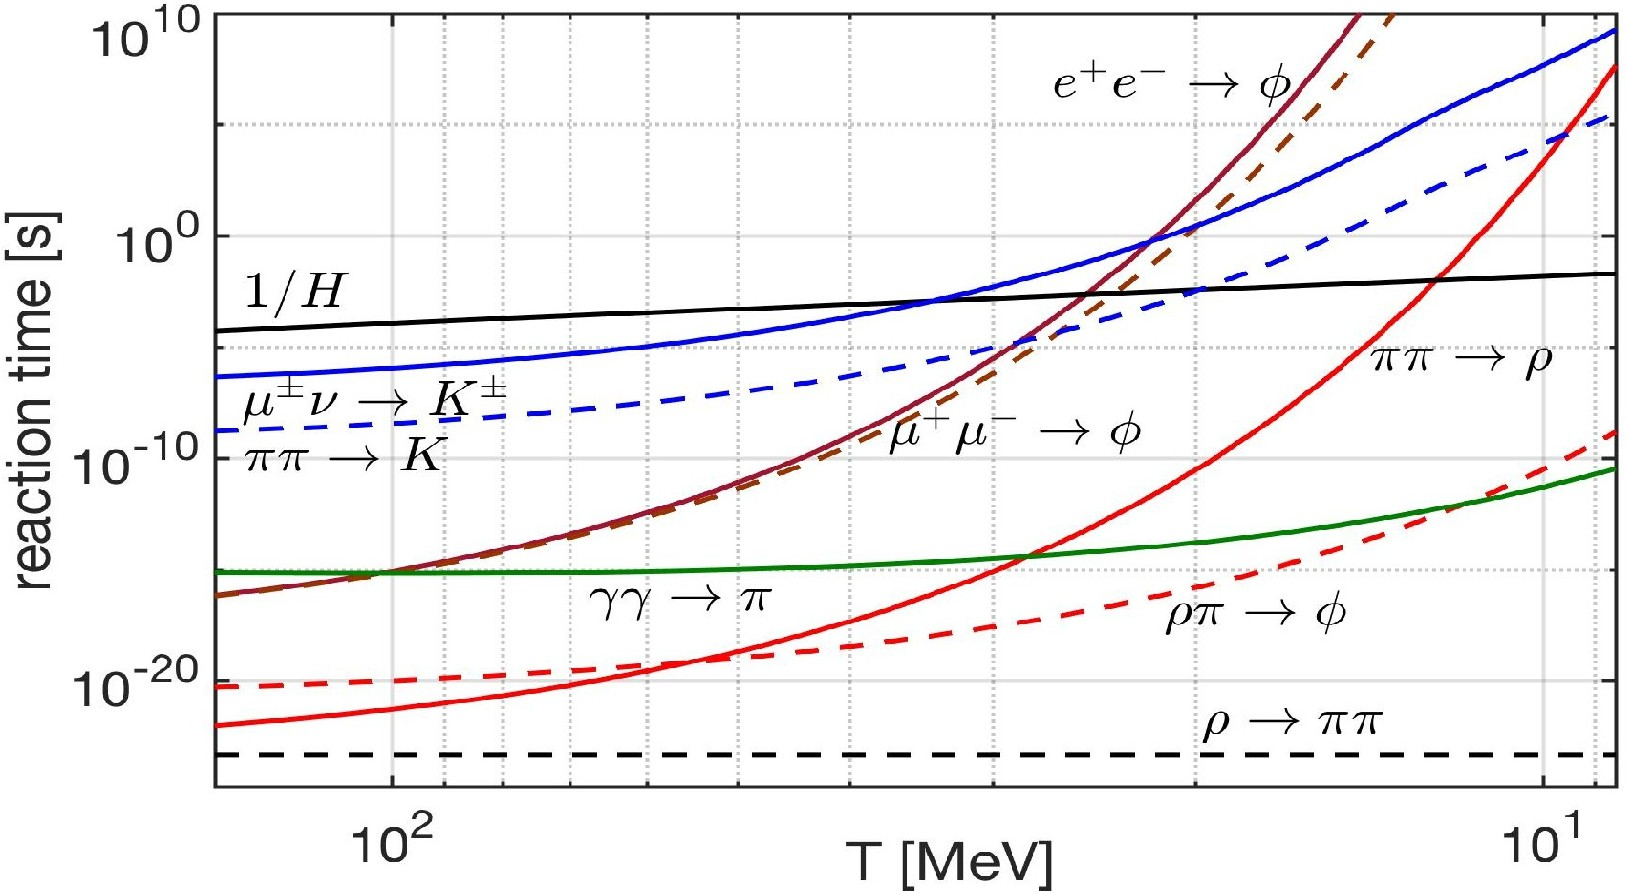
\includegraphics[width=0.95\linewidth]{./plots/Strangeness_Hubble_C.jpg}
\centerline{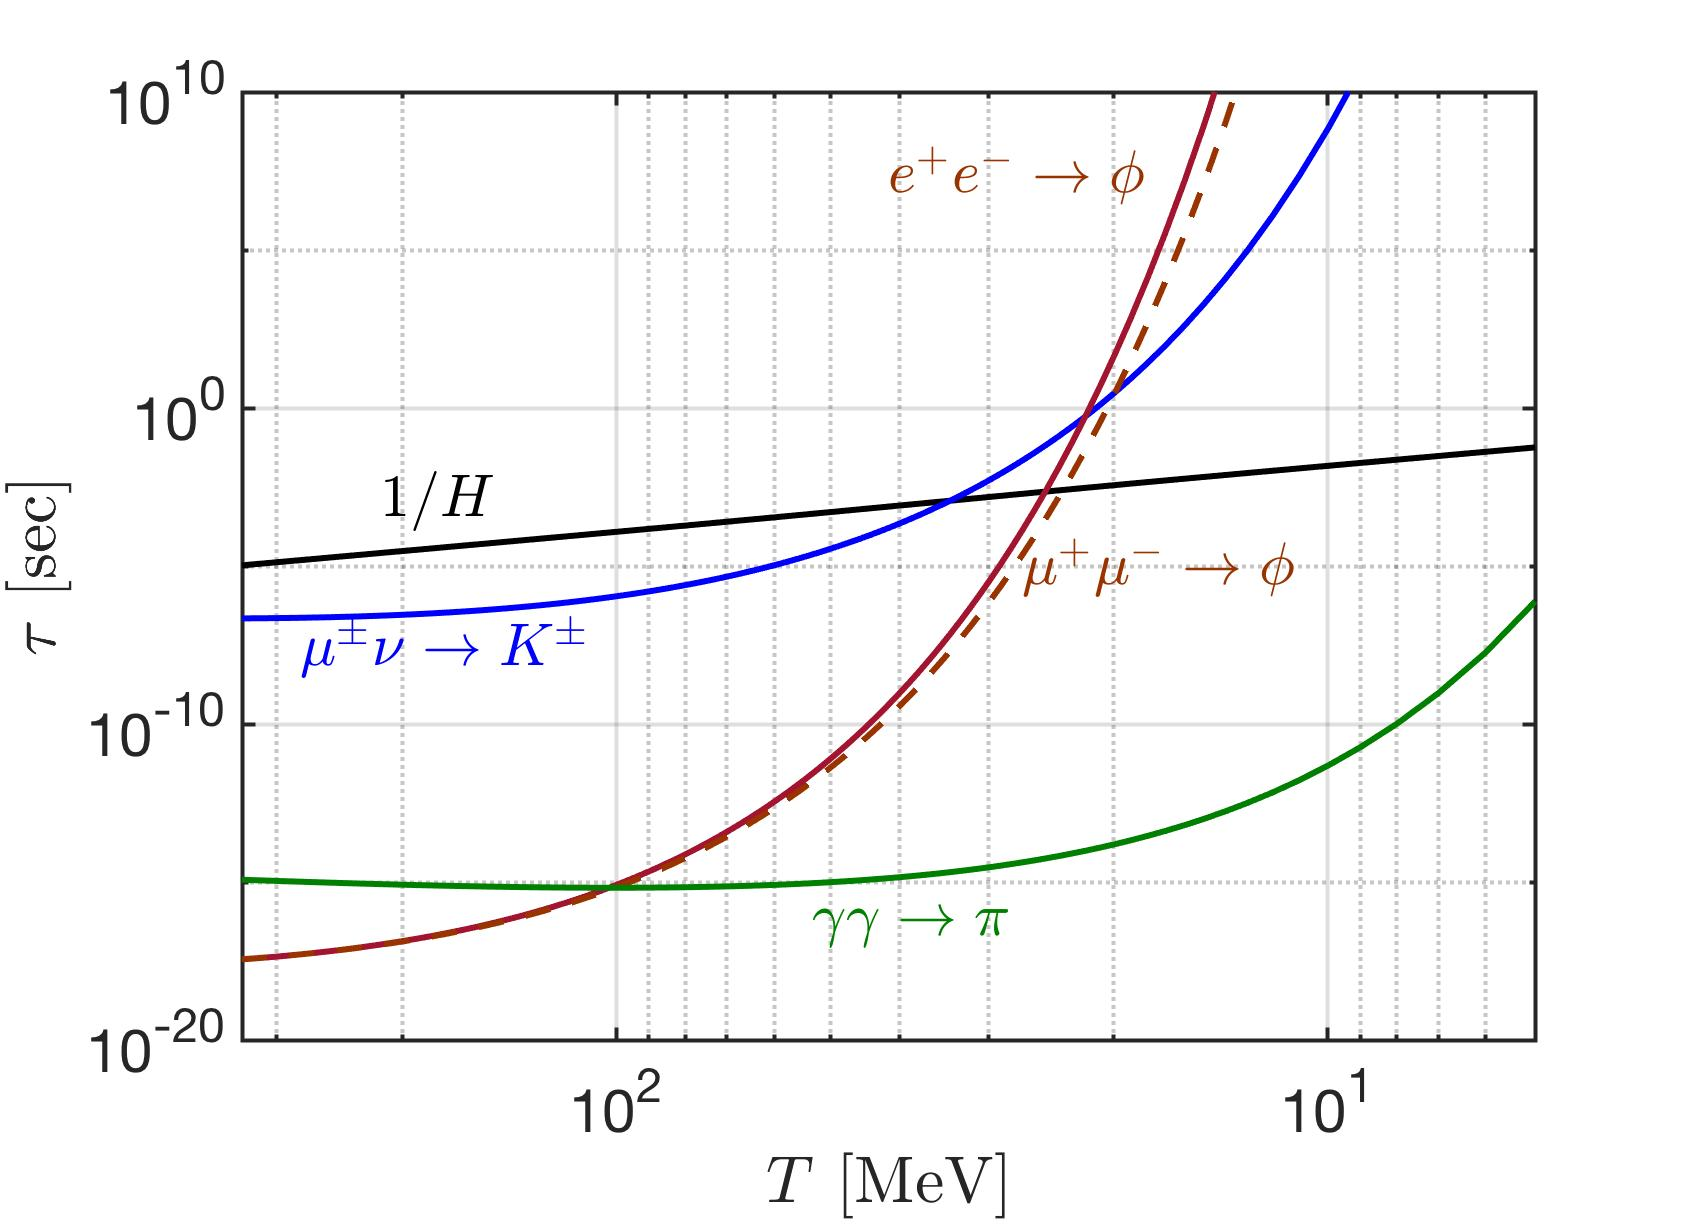
\includegraphics[width=0.9\linewidth]{./plots/Strangeness_Hubble002.jpg}}
\centerline{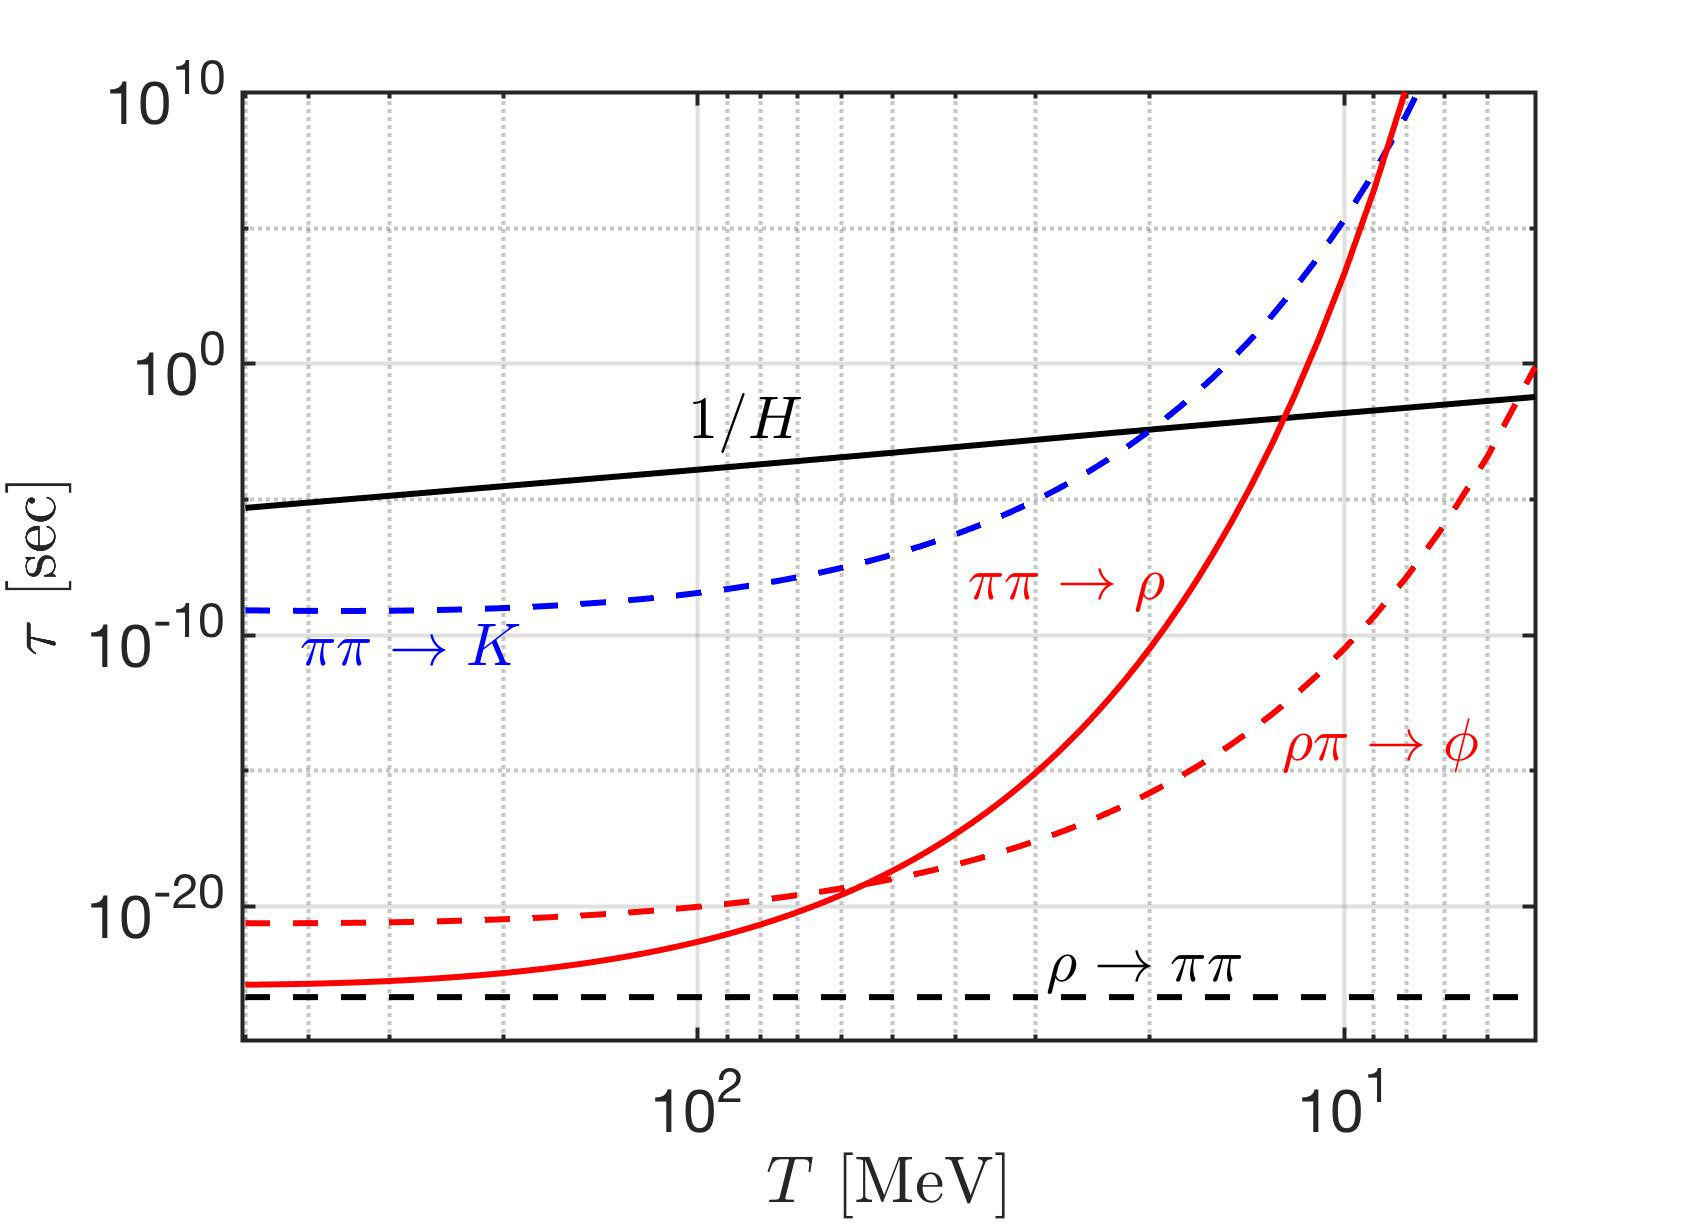
\includegraphics[width=0.9\linewidth]{./plots/Strangeness_Hubble003.jpg}}
\caption{\cccite{Rafelski:2023emw}, adapted from Ref.~\cite{Yang:2021bko} and thesis of C.T.Yang \cite{Yang:2024ret}. Hadronic relaxation reaction times, see Eq.\,(\ref{Reaction_Time}), as a function of temperature $T$, are compared to Hubble time $1/H$ (black solid line). At bottom the horizontal black-dashed line is the natural (vacuum) lifespan of $\rho$}
\label{reaction_time_tot} 
\end{figure}
%%%%%%%%%%%%%%%%%%%%%%%%

In \rf{reaction_time_tot} we plot the  hadronic reaction relaxation times $\tau_{i}$ in the meson sector as a function of temperature compared to Hubble time $1/H$. We note that the weak interaction reaction $\mu^\pm+\nu_{\mu}\rightarrow K^\pm$ becomes slower compared to the Universe expansion near temperature $T_f^{K^\pm}=33.8\,\mathrm{MeV}$, signaling the onset of abundance nonequilibrium for $K^\pm$. For $T<T_f^{K^\pm}$, the reactions $\mu^\pm+\nu_{\mu}\rightarrow K^\pm$ decouples from the cosmic plasma; the corresponding detailed balance can be broken and the decay reactions $K^\pm\rightarrow\mu^\pm+\nu_{\mu}$ are acting like a (small) ``hole'' in the strangeness abundance ``pot''. If other strangeness production reactions did not exist, strangeness would disappear as the Universe cools below $T_f^{K^\pm}$.  However, there are other reactions: $l^++l^-\leftrightarrow\phi$, $\pi+\pi\leftrightarrow K$, and $\rho+\pi\leftrightarrow\phi$ can still produce the strangeness in cosmic plasma and the rate is very large compared to the weak interaction decay.


In Table~\ref{FreezeoutTemperature_table} we also show the characteristic strangeness reactions and their freeze-out temperatures in the early Universe. The intersection of strangeness reaction times with $1/H$ occurs for $l^-+l^+\rightarrow\phi$ at $T_f^\phi=25\sim23\,\mathrm{MeV}$, and for $\pi+\pi\rightarrow K$ at $T_f^K=19.8\,\mathrm{MeV}$, for $\pi+\pi\rightarrow\rho$ at $T_f^\rho=12.3\,\mathrm{MeV}$. The reactions $\gamma+\gamma\rightarrow\pi$ and $\rho+\pi\leftrightarrow\phi$ are faster compared to $1/H$. However, the $\rho\to\pi+\pi$ lifetime (black dashed line in \rf{reaction_time_tot}) is smaller than the reaction $\rho+\pi\leftrightarrow\phi$; in this case, most of $\rho$-meson decays faster, thus are absent and cannot contribute to the strangeness creation in the meson sector. Below the temperature $T<20$\,MeV, all the detail balances in the strange meson reactions are broken and the strangeness in the meson sector should disappear rapidly, were it not for the small number of baryons present in the Universe.

%%%%%%%%%%%%%%%%%%%%%%%%%%%%%%%%%%%%%%%%%%%%
\paragraph{Strangeness production and exchange rates in hyperons}
In order to understand strangeness in hyperons in the baryonic domain, we now consider the strangeness production reaction $\pi +N\rightarrow K+\Lambda$, the strangeness exchange reaction $\overline{K}+N\rightarrow \Lambda+\pi$; and the strangeness decay $\Lambda\rightarrow N+\pi$. The competition between different strangeness reactions allows strange hyperons and antihyperons to influence the dynamic nonequilibrium condition, including development of $\langle s-\bar s\rangle \ne 0$. %The cross sections $\sigma_{\overline{K}N\rightarrow \Lambda\pi}$ and $\sigma_{\pi N\rightarrow K\Lambda}$ are obtained from experiment.

To evaluate the reaction rate in two-body reaction $1+2\rightarrow3+4$ in the Boltzmann approximation we can use the reaction cross section $\sigma(s)$ and the relation~\cite{Letessier:2002ony}:\index{hyperon!production rate}
\begin{align}
R_{12\rightarrow34}=\frac{g_1g_2}{32\pi^4}\frac{T}{1+I_{12}}\!\!\int^\infty_{s_{th}}\!\!\!\!ds\,\sigma(s)\frac{\lambda_2(s)}{\sqrt{s}}\!K_1\!\!\left({\sqrt{s}}/{T}\right),
\end{align}
where $K_1$ is the Bessel function of order $1$ and the function $\lambda_2(s)$ is defined as
\begin{align}
\lambda_2(s)=\left[s-(m_1+m_2)^2\right]\left[s-(m_1-m_2)^2\right],
\end{align}
with $m_1$ and $m_2$, $g_1$ and $g_2$ as the masses and degeneracy of the initial interacting particle. The factor $1/(1+I_{12})$ is introduced to avoid double counting of indistinguishable pairs of particles; we have $I_{12}=1$ for identical particles and $I_{12}=0$ for others. 

The thermal averaged cross sections for the strangeness production and exchange processes are about $\sigma_{\pi N\rightarrow K\Lambda}\sim0.1\,\mathrm{mb}$ and $\sigma_{\overline{K}N\rightarrow \Lambda\pi}=1\sim3\,\mathrm{mb}$ in the energy range in which we are interested~\cite{Koch:1986ud}. The cross section can be parameterized as follows:\\
1) For the cross section $\sigma_{\overline{K}N\rightarrow \Lambda\pi}$ we use~\cite{Koch:1986ud}
 \begin{align}
 \sigma_{\overline{K}N\rightarrow \Lambda\pi}=\frac{1}{2}\left(\sigma_{K^-p\rightarrow \Lambda\pi^0}+\sigma_{K^-n\rightarrow \Lambda\pi^-}\right)\,.
\end{align}
Here the experimental cross sections can be parameterized as 
\begin{align}
&\sigma_{K^-p\rightarrow \Lambda\pi^0}\!\!=\!\!\left(\begin{array}{l}\!\!1479.53\mathrm{mb}\!\cdot\!\exp{\left(\frac{-3.377\sqrt{s}}{\mathrm{GeV}}\right)},\; \mathrm{for}\,\sqrt{s_m}\!\!<\!\!\sqrt{s}\!<\!3.2\mathrm{GeV} \\ \\0.3\mathrm{mb}\!\cdot\!\exp{\left(\frac{-0.72\sqrt{s}}{\mathrm{GeV}}\right)},\; \mathrm{for}\sqrt{s}>3.2\mathrm{GeV}\end{array}\right.\\
&\sigma_{K^-n\rightarrow \Lambda\pi^-}\!\!=\!\!1132.27\mathrm{mb}\!\cdot\!\exp{\left(\frac{-3.063\sqrt{s}}{\mathrm{GeV}}\right)},\; \mathrm{for}\sqrt{s}>1.699\mathrm{GeV},
\end{align}
where $\sqrt{s_m}=1.473$ GeV.\\
2) For the cross section $\sigma_{\pi N\rightarrow K\Lambda}$ we use~\cite{Cugnon:1984pm}
\begin{align}
&\sigma_{\pi N\rightarrow K\Lambda}=\frac{1}{4}\times\sigma_{\pi p\rightarrow K^0\Lambda}\,.
\end{align}
The experimental $\sigma_{\pi p\rightarrow K^0\Lambda}$  can be approximated as follows
\begin{align}
\sigma_{\pi p\rightarrow K^0\Lambda}=\left(\begin{array}{l}\frac{0.9\mathrm{mb}\cdot\left(\sqrt{s}-\sqrt{s_0}\right)}{0.091\mathrm{GeV}},\; \mathrm{for} \sqrt{s_0}<\sqrt{s}<1.7\mathrm{GeV} \\ \\ \frac{90\mathrm{MeV\cdot mb}}{\sqrt{s}-1.6\mathrm{GeV}},\; \mathrm{for}\sqrt{s}>1.7\mathrm{GeV},\end{array}\right.
 \end{align}
 with $ \sqrt{s_0}=m_\Lambda+m_K$. 

Given the cross sections, we obtain the thermal reaction rate per volume for strangeness exchange reaction seen in \rf{Lambda_Rate_volume.fig}. We see that around $T=20$\,MeV, the dominant reactions for the hyperon $\Lambda$ production is $\overline{K}+N\leftrightarrow\Lambda+\pi$. At the same time, the $\pi+\pi\to K$ reaction becomes slower than Hubble time and kaon $K$ decay rapidly in the early Universe. However, the anti-kaons $\overline K$ produce the hyperon $\Lambda$ because of the strangeness exchange reaction $\overline{K}+N\rightarrow\Lambda+\pi$ in the baryon-dominated Universe. We have strangeness in $\Lambda$ and it disappears from the Universe via the decay $\Lambda\rightarrow N+\pi$. Both strangeness and anti-strangeness disappear because of the $K\rightarrow\pi+\pi$ and $\Lambda\rightarrow N+\pi$, while the strangeness abundance $s = \bar{s}$ in the early Universe remains.

%%%%%%%%%%%%%%%%%%%%%%%%%%%%%%%%
\begin{figure} 
\centerline{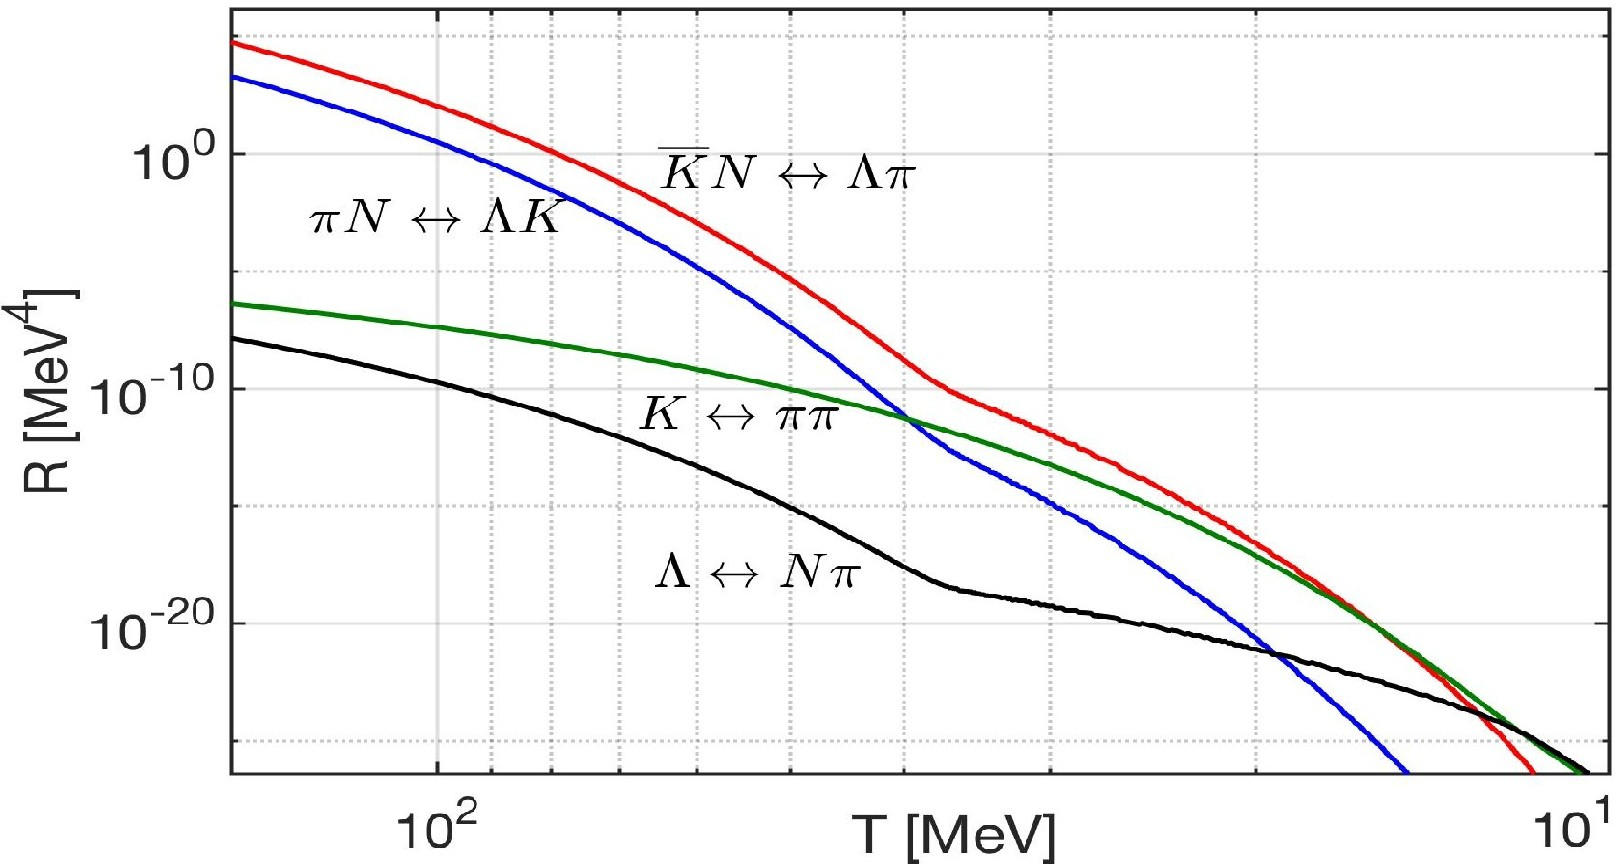
\includegraphics[width=0.9\linewidth]{./plots/NewHyperonRate_C.jpg}}
\caption{\cccite{Rafelski:2023emw}, adapted from Ref.~\cite{Yang:2021bko} and thesis of C.T.Yang \cite{Yang:2024ret}. Thermal reaction rate $R$ per volume and time for important hadronic strangeness production and exchange processes as a function of temperature $150\,\mathrm{MeV}> T>10\,\mathrm{MeV}$ in the early Universe}
\label{Lambda_Rate_volume.fig} 
\end{figure}
%%%%%%%%%%%%%%%%%%%%%%%%%%%%%%%%%%%%

Near to $T=12.9$\,MeV  the reaction $\Lambda+\pi\rightarrow\overline{K}+N$ becomes slower than the strangeness decay $\Lambda\leftrightarrow N+\pi$ and shows that at the low temperature the $\Lambda$ particles are still in equilibrium via the reaction $\Lambda\leftrightarrow N+\pi$ and little strangeness remains in the $\Lambda$. Then strangeness abundance becomes asymmetric $s\gg \bar{s}$, which implies that the assumption for strangeness conservation can only be valid until the temperature $T\sim13$\,MeV. Below this temperature a new regime opens up in which the tiny residual strangeness abundance is governed by weak decays with no re-equilibration with mesons. Also, in view of baron asymmetry, $\langle s-\bar s\rangle \ne 0$.

The main conclusion of this first study of strangeness production and content in the early Universe, following on QGP hadronization, is that the relevant temperature domains indicate a complex interplay between baryon and meson (strange and non-strange) abundances and non-trivial decoupling from equilibrium for strange and non-strange mesons. We believe that this work contributes to the opening of a new and rich domain in the study of the Universe evolution in the future. 
